\documentclass[a4paper, oneside]{discothesis}

\usepackage[utf8]{inputenc}
\usepackage[T1]{fontenc}
\usepackage{bbm}
\usepackage{algorithm}
\usepackage{algpseudocode}
\usepackage{xcolor}
\usepackage{bm}
\usepackage{booktabs}
\usepackage{mathtools} 
\usepackage{csvsimple}
\usepackage{multirow}
\usepackage{amsmath}
\setcounter{secnumdepth}{3}
\usepackage{biblatex}
\usepackage{graphics}
\usepackage{diagbox}
\usepackage{lmodern}
\usepackage{mdframed}
\usepackage{multicol}





\addbibresource{references.bib}



%%%%%%%%%%%%%%%%%%%%%%%%%%%%%%%%%%%%%%%%%%%%%%%%%%%%%%%%%%%%%%%%%%%%%%%%%%%%%%%%%%%%%%%%%%%%%%%%%
% DOCUMENT METADATA

\thesistype{Master Thesis\\ MSc Quantitative Finance ETH/UZH} % Master's Thesis, Bachelor's Thesis, Semester Thesis, Group Project
\title{Comparison of Statistical and Machine Learning Methods in Modelling Time-Varying Volatility 
}

\author{Georgios Avgoustinos}
\email{georgios.avgoustinos@uzh.ch}

\institute{Department of Banking and Finance\\
University of Zurich}

% Optionally, you can put in your own logo here
%\logo{
\includegraphics[width=0.2\columnwidth]{figures/disco_logo_faded}}

\supervisors{Prof. Dr. Erich Walter Farkas\\
 Zaid Siddiqi (\textit{Zanders Treasury \& Risk})}

% Optionally, keywords and categories of the work can be shown (on the Abstract page)
%\keywords{Keywords go here.}
%\categories{ACM categories go here.}

\date{\today}

%%%%%%%%%%%%%%%%%%%%%%%%%%%%%%%%%%%%%%%%%%%%%%%%%%%%%%%%%%%%%%%%%%%%%%%%%%%%%%%%%%%%%%%%%%%%%%%%%

\begin{document}

\frontmatter % do not remove this line
\maketitle

\cleardoublepage

\begin{acknowledgements}
	I thank Lorem ipsum dolor sit amet, consetetur sadipscing elitr, sed diam nonumy eirmod tempor invidunt ut labore et dolore magna aliquyam erat, sed diam voluptua. At vero eos et accusam et justo duo dolores et ea rebum. Stet clita kasd gubergren, no sea takimata sanctus est Lorem ipsum dolor sit amet. Lorem ipsum dolor sit amet, consetetur sadipscing elitr, sed diam nonumy eirmod tempor invidunt ut labore et dolore magna aliquyam erat, sed diam voluptua. At vero eos et accusam et justo duo dolores et ea rebum. Stet clita kasd gubergren, no sea takimata sanctus est Lorem ipsum dolor sit amet.
\end{acknowledgements}


\begin{abstract}
    The abstract should be short, stating what you did and what the most important result is.
	Lorem ipsum dolor sit amet, consetetur sadipscing elitr, sed diam nonumy eirmod tempor invidunt ut labore et dolore magna aliquyam erat, sed diam voluptua. At vero eos et accusam et justo duo dolores et ea rebum. Stet clita kasd gubergren, no sea takimata sanctus est Lorem ipsum dolor sit amet. Lorem ipsum dolor sit amet, consetetur sadipscing elitr, sed diam nonumy eirmod tempor invidunt ut labore et dolore magna aliquyam erat, sed diam voluptua. At vero eos et accusam et justo duo dolores et ea rebum. Stet clita kasd gubergren, no sea takimata sanctus est Lorem ipsum dolor sit amet.
\end{abstract}

\tableofcontents

\mainmatter % do not remove this line

% Start writing here
\chapter{Introduction}
\todo[]{all $t=1, 2, \dots$ to be changed with $t\in\mathbb{N}$}
\todo[]{every equation numbered}

\chapter{Literature Overview of Statistical Volatility Models}

\section{One Dimensional Models}\label{one_d}
\todo[]{More details in the specification of Garch, Egarch, GJR. Some remarks and probably unconditional variance or forecasting close form.}
Standard methods for a statistical modelling of financial returns include linear regression or Auto-regressive Moving Averages (ARMA)  models. Though, their main assumption is the existence of homoskedasticity on the residuals meaning a constant volatility throughout time, which do not seem to agree with the empirical findings. For instance, the authors in \cite{QRM} observe some stylized facts in financial returns and among others, they highlight that:
\begin{itemize}
    \item Return series are not iid although they show little serial correlation.
    \item Volatility appears to vary over time.
    \item  Extreme returns appear in clusters.
\end{itemize}

In that regard and to deal with the mentioned characteristics, in the specific section we will focus on modelling conditional volatility in one dimensional time series of returns.

We will introduce three important statistical models widely used for volatility modelling. After that, we will describe the problem formulation with the methodology used and the different models used. Finally, we will provide a detailed comparison of the studied models. The main objective is to introduce to the reader three cornerstone statistical models that will be later used as baseline models. 

To put things formally, we work in a usual probability triplet $\left( \Omega, \mathcal{F}, \mathbb{P}\right)$ equipped with the filtration $\mathbb{F} = \left(\mathcal{F}_t\right)_{t = 1, 2, \dots}$ which is generated by the available information of the market at each time step. We denote the asset's returns with the $\mathbb{F}$-adapted process  $\left(x_t\right)_{t = 1, 2, \dots}$ and our main assumption is that for $t = 1,2,\dots$ 

\begin{equation}\label{eq:1d-ass}
x_t \sim \mathcal{N}\left(\mu, \sigma_t\right)
\end{equation}

where $\sigma_t$ is a $\mathbb{F}$-predictable stochastic process denoting the conditional volatility at each time step.




  \begin{mdframed}\begin{remark}
We choose to consider the mean of the returns constant over time as we mainly focus on modelling the conditional volatility. Moreover, in the model specification and implementation later, the mean will be considered to be $0$, which is a popular choice in both single and multiple dimensions (see later) used in \cite{boulet}, \cite{fgd}, \cite{engle-multidimensions} among many others.
\end{remark}\end{mdframed}  

  \begin{mdframed}\begin{remark}
Without loss of generality, we decide to continue with the assumption that the conditional returns are normally distributed, even though Students-t extensions exist in the literature \cite{garch-t}.
\end{remark}\end{mdframed}  


\subsection{GARCH}

Generalized Autoregressive Conditional Heteroskedastic model was introduced by the author \cite{garch} and can be considered to be the starting point of volatility modelling.

\begin{definition}[GARCH $\left(p, q\right)$]\label{thm:garch_def}

$\left(x_t\right)_{t\in \mathbb{N}}$ follows a normal GARCH $\left(p, q\right)$ process with zero mean, if $\forall t \in \mathbb{N}$ holds that

\begin{gather*}\label{eq:1}
x_t = \sigma_t \epsilon_t \\
\sigma^2_t = \omega + \sum_{i=1}^p\alpha_i x_{t-i}^2 + \sum_{j=1}^q \beta_j 
\sigma_{t-j}^2  \\
\epsilon_t \sim \mathcal{N}\left(0,1\right)
\end{gather*}

\end{definition}
where $\omega > 0, \alpha_i \geq 0, i = 1,\dots,p$ and $\beta_j \geq 0, j = 1,\dots,q$

Even though, the model is simple enough, it is able to capture important features of financial returns data such as the volatility clustering. On the other hand due to the symmetry in the formula the \textit{leverage effect} cannot be captured and both upward and downward movements of the market seem to affect the volatility in the same way.

The parameters $p$ and $q$ are noting the time lag of the returns and volatility respectively.

\subsection{EGARCH}

The author \cite{egarch} introduced the exponential GARCH model as a further extension of \ref{thm:garch_def}  to deal with the leverage feature.

\begin{definition}[EGARCH $\left(p, q\right)$]\label{thm:egarch_def} $\left(x_t\right)_{t\in \mathbb{N}}$ follows a normal EGARCH $\left(p, q\right)$ process with zero mean, if $\forall t \in \mathbb{N}$ holds that

\begin{gather*}\label{eq:}
x_t = \sigma_t \epsilon_t \\
\log\sigma^2_t = \omega + \sum_{i=1}^p\alpha_i \left(|\epsilon_{t-i}|+\gamma_i\epsilon_{t-i}\right) + \sum_{j=1}^q \beta_j \log \sigma_{t-j}^2  \\
\epsilon_t \sim \mathcal{N}\left(0,1\right)
\end{gather*}

\end{definition}
where the $\gamma_i$ parameters signifies the asymmetric effects from $x_{t-i}$. 

\subsection{GJR}

In continuation with the aim of capturing better the leverage effect, the authors \cite{gjr} suggested the Glosten-Jagannathan-Runkle GARCH model. 

\begin{definition}[GJR]\label{thm:gjr} 
$\left(x_t\right)_{t\in \mathbb{N}}$ follows a normal GJR process with zero mean, if $\forall t \in \mathbb{N}$ holds that

\begin{gather*}\label{eq:}
x_t = \sigma_t \epsilon_t \\
\sigma^2_t = \omega + \left(\alpha+\gamma \mathbbm{1}_{x_{t-1}<0}\right)x_{t-1}^2+\beta \sigma_{t-1}^2 \\
\epsilon_t \sim \mathcal{N}\left(0,1\right)
\end{gather*}
\end{definition}


\subsection{Model Estimation}

For the parameter estimation of the mentioned models the method which is used is \textit{Maximum Likelihood Estimation (MLE)}.

More precisely, we denote the returns vector by $\mathbf{X}$ and without loss of generality we may consider time lag of one step. 
\begin{equation}
    f_{\bm{X}}(x_1, \dots, x_n) = f_{X_1}(x_1)\prod_{t=1}^{n-1}f_{X_{t+1}|X_t}(x_{t+1}|x_t)
\end{equation}


Denoting by $\bm{\theta}$ the model parameters, one can write the conditional variance in a general form of $\sigma_t^2 = g(\bm{\theta}, x_{t-1})$ for a measurable function $g$ which is determined from the specific model. 

Switching to the log-prices, one has
\begin{equation}
    L\left(\bm{\theta}| \bm{X}\right) = \log f_{\bm{X}}(x_1, \dots, x_n) = \log f_{X_1}(x_1) + \sum_{t=1}^{n-1} \log  f_{X_{t+1}|X_t}(x_{t+1}|x_t) 
\end{equation}

According to the normal zero-mean assumption of the returns,

\begin{equation}
\begin{split}
      L\left(\bm{\theta}| \bm{X}\right) = -\frac{1}{2}\sum_{t=1}^n \log(2\pi)+\log(\sigma_t^2)+\frac{x_t^2}{\sigma_t^2}=\\-\frac{1}{2}\left(n\log(2\pi)+\sum_{t=1}^n \log(g(\bm{\theta}, x_{t-1}))+\frac{x_t^2}{g(\bm{\theta}, x_{t-1})}\right)
\end{split}
\end{equation}

thereby, the optimal parameters can be viewed as solutions to the optimization problem:

\begin{equation}
    \bm{\theta}^* = \underset{\bm{\theta}}{\mathrm{argmin }} -L\left(\bm{\theta}| \bm{X}\right)
\end{equation}

The optimal parameters in general are a local maximum and solve the equations

\begin{equation}\label{eq:scores}
    \frac{\partial}{\partial\bm{\theta}}L\left(\bm{\theta}| \bm{X}\right) = 0
\end{equation}

where the left-hand side is known as the \textit{score vector}.  

The equation \ref{eq:scores} is solved numerically with Newton-Raphson methods. The one most typically used is the BHHH \cite{bhhh} method.

\section{Multidimensional Models}

Capturing the dependence structure of a portfolio's returns is an important manner in the fields of Asset and Risk Management. Especially, after the publication of \cite{MPT}, which signaled the start of Modern Portfolio Theory, researchers began focusing in the observation and estimation of return's covariances. 

Though, under the time varying volatility assumption the estimation of a covariance matrix in multiple dimensions and for every time step leads to huge computational complexity and inefficiency. The specific occurring problem is referred as ``curse of dimensionality'' and it stands as the main reason why the volume of studies in the multidimensional case is significantly smaller compared to the one-dimensional case.

To deal with it, the most widely used assumption from the researchers is that a part of the dependency remains the same whereas another one changes according to recursive equations similar to the one-dimensional approach.

To what follows, we will focus on the \textit{Conditional Correlation} multivariate GARCH models which stand as a simplified extension of the one-dimensional GARCH models to multiple dimensions. The specific models are also seemingly efficient during estimation especially when the number of assets is large.

In more detail, assuming that a portfolio is consisted of $d$ assets, we can again work in a probability triplet $(\Omega, \mathcal{F}, \mathbb{P})$ and denote the assets' returns as a $d$-valued stochastic process $\mathbf{X} = (\mathbf{X}_t)_{t\in\mathbb{N}}$ and the filtration generated from them as $\mathbb{F} = (\mathcal{F})_{t\in\mathbb{N}}$. Then $\bf{X}$ is stated to follow a \textit{Conditional Correlation}-Garch process with Gaussian innovations if it is of the following form.

\begin{gather}
    \mathbf{X}_t|\mathcal{F}_{t-1}\sim\mathcal{N}(0, \Sigma_t)\label{eq: mgarch1}\\
    \Sigma_t = \Delta_t P_t \Delta_t\\
    \Delta_t = \text{diag}(\sigma_{t, 1}, \dots, \sigma_{t,p})\\
    \begin{split}\label{eq: mgarch2}
    \sigma_{t, k}^2 = \alpha_{k0}+\sum_{i=1}^{p_k}\alpha_{ki}X^2_{t-i, k}+\sum_{j=1}^{q_k}\beta_{kj}\sigma^2_{t-j, k}\text{, for }k\in\{1,\dots ,d \}\\ \text{where, } \alpha_{k0} \geq 0\text{, } \alpha_{ki}\geq0, i\in\{1, \dots, p_k\}\text{ and } \beta_{kj}\geq0, j\in\{1, \dots, q_k\}
    \end{split}\\
    P_t = f(\mathcal{F}_{t-1})
\end{gather}
for $t\in \mathbb{N}$ and a measurable function $f$ that maps to the measurable space $\left( \mathbb{R}^{d\times d}, \mathcal{B}_{\mathbb{R}^{d\times d}} \right)$.

\subsection{CCC-GARCH}
The \textit{Constant Conditional Correlation} (CCC) model was introduced by \cite{CCC} and stands as a first main attempt for modelling portfolio returns in multiple dimensions.

\begin{definition}[CCC-GARCH]
The $d$-valued stochastic process $(\mathbf{X}_t)_{t\in\mathbb{N}}$ is a CCC-GARCH process if (i) it follows the form stated in the equations \ref{eq: mgarch1}-\ref{eq: mgarch2} and (ii) $P_t = P_c$, for $t\in \mathbb{N}$, where $P_c\in\mathbb{R}^{d\times d}$ is constant correlation matrix. 
\end{definition}

  \begin{mdframed}\begin{remark}
The model is well defined as the covariance matrix is always positive definite. Note that $\forall \mathbf{x}\neq\mathbf{0}\in\mathbb{R}^d$ one has:
\[\mathbf{x}^\intercal\Sigma_t\mathbf{x} = \left(\Delta_t\mathbf{x}\right)^\intercal P_c \left(\Delta_t\mathbf{x}\right)>0\]
since $P_c$ is a positive definite matrix and the individual volatilities $\sigma_{t, \cdot}$ that compose $\Delta_t$ are strictly positive.
\end{remark}\end{mdframed}  
In general, CCC is a useful baseline model. Though, due to its simplicity it seems to not capture well features of the market. For instance, the impact of news in the market forces a model to have a dynamic relationship for the correlation matrix which is in contrast with the CCC model.

The estimation of the model is rather simple as well and it can be performed in two steps. An useful notation for the estimation procedure is this of the \textit{devolatized} returns $\mathbf{Y}_t \coloneqq \Delta_t^{-1}\mathbf{X}_t$ as $\mathbf{Y}_t\sim \mathcal{N}(0, P_c)$.

\begin{algorithm}
\caption{Estimation of CCC model}
\begin{algorithmic}
\State \begin{enumerate}
    \item Fit $d$ individual GARCH models for each asset to estimate $\sigma_{t, k}, \forall t\in \{1, \dots, T\},\forall k\in\{1, \dots, d\}$
    \item Calculate the \textit{devolitized} returns $\mathbf{Y}_t = \Delta_t^{-1}\mathbf{X}_t$ and estimate $P_c$ as their covariance matrix, $P_c = \frac{1}{T}\sum_{t=1}^T \mathbf{Y}_t\mathbf{Y}_t^\intercal$.
\end{enumerate}
\end{algorithmic}
\end{algorithm}

\subsection{DCC-GARCH}
\textit{Dynamic Conditional Correlation} (DCC) model was introduced by \cite{DCC} and stands as a more realistic extension of CCC as the correlation matrix evolves recursively. 

For a mathematical definition of the model, it is important to define a function $\mathfrak{P}: \mathbb{R}^{d\times d}\mapsto\mathbb{R}^{d\times d}$ that maps covariance matrices to correlation matrices as follows:
\begin{equation}
    M \longmapsto\mathfrak{P}(M) = \text{diag}\left(\frac{1}{M_{1,1}}, \dots, \frac{1}{M_{d,d}}\right)M  \text{diag}\left(\frac{1}{M_{1,1}}, \dots, \frac{1}{M_{d,d}}\right)
\end{equation}
\begin{definition}[DCC-GARCH]
The $d$-valued stochastic process $(\mathbf{X}_t)_{t\in\mathbb{N}}$ is a DCC-GARCH process if:
\begin{enumerate}
    \item  It follows the form stated in the equations \ref{eq: mgarch1}-\ref{eq: mgarch2}
    \item $P_t = \mathfrak{P}(Q_t) \text{, }\forall t\in\mathbb{N}$, with 
    \begin{gather}
        Q_t\coloneqq \left(1-\sum_{i=1}^p \alpha_i - \sum_{j=1}^q \beta_j\right)P_c+\sum_{i=1}^p\alpha_i\mathbf{Y}_{t-i}\mathbf{Y}_{t-i}^\intercal + \sum_{j=1}^q\beta_j P_{t-j}\\\mathbf{Y}_t= \Delta_t^{-1}\mathbf{X}_t\text{   (the \textit{devolatized} returns)}\\
        P_c = \frac{1}{T}\sum_{t=1}^T \mathbf{Y}_t\mathbf{Y}_t^\intercal\text{   (the constant correlation matrix)}
    \end{gather}
\end{enumerate}
\end{definition}
  \begin{mdframed}\begin{remark}
Note that the matrices $(Q_t)_{t\in\mathbb{N}}$ are well defined positive definite covariance matrices iff $\sum_{i=1}^p \alpha_i + \sum_{j=1}^q \beta_j<1$. In more detail,  $\forall \mathbf{x}\neq\mathbf{0}\in\mathbb{R}^d$ one has:
\scriptsize
\[\mathbf{x}^\intercal Q_t\mathbf{x} = \left(1-\sum_{i=1}^p \alpha_i - \sum_{j=1}^q \beta_j\right)\mathbf{x}^\intercal P_c\mathbf{x}+\sum_{i=1}^p\alpha_i\mathbf{x}^\intercal\mathbf{Y}_{t-i}\mathbf{Y}_{t-i}^\intercal\mathbf{x} + \sum_{j=1}^q\beta_j \mathbf{x}^\intercal P_{t-j}\mathbf{x}>0\]\[\Longleftrightarrow\]\[\sum_{i=1}^p \alpha_i + \sum_{j=1}^q \beta_j<1\]
\end{remark}\end{mdframed}  
\normalsize

Regarding the fitting of DCC model in data, maximum likelihood methods is widely used. Although, someone can directly estimate all of the parameters in one step via MLE, the most common approach is the estimation in two steps, one for the individual volatilities and one for the estimation of the conditional correlations. 

  \begin{mdframed}\begin{remark}
For the determination of the objective function for optimization, recall that the negative log-likelihood for Gaussian residuals in a dataset $\mathbf{x} = (\mathbf{x}_t)_{t=1}^T$ is been given from:
\[l_{\mathbf{X}}(\mathbf{x}) = \frac{1}{2}\sum_{t-1}^T d\log2\pi+\log|\Sigma_t|+\mathbf{x}_t^\intercal\Sigma_t^{-1}\mathbf{x}_t\]
and according to the assumptions of the model, one has
\[l_{\mathbf{X}}(\mathbf{x}) = \frac{1}{2}\sum_{t-1}^T d\log2\pi+2\log|\Delta_t|+\log|P_t|+(\Delta_t^{-1}\mathbf{x}_t)^\intercal P_t^{-1}(\Delta_t^{-1}\mathbf{x}_t)\]
removing now the constant terms (including the individual volatilities) and switching to the \textit{devolitized} returns' notation we can define a loss function as follows:
\begin{equation}\label{eq: loss_dcc}
    L(y| \boldsymbol{\theta}) \coloneqq \sum_{t-1}^T \log|P_t(\boldsymbol{\theta})|+\mathbf{y}_t^\intercal P_t(\theta)^{-1}\mathbf{y}_t
\end{equation}
where $\boldsymbol{\theta} = (\alpha_1, \dots, \alpha_p, \beta_1, \dots, \beta_q)$.
\end{remark}\end{mdframed}  

Summarizing all of the above, the estimation of the model can be described in what follows.
\begin{algorithm}
\caption{Estimation of DCC model}
\begin{algorithmic}
\State\begin{enumerate}
    \item Fit $d$ individual GARCH models for each asset to estimate $\sigma_{t, k}, \forall t\in \{1, \dots, T\},\forall k\in\{1, \dots, d\}$.
    \item Calculate the \textit{devolitized} data $\mathbf{y}_t = \Delta_t^{-1}\mathbf{x}_t$ and estimate $P_c$ as their covariance matrix. 
    \item Solve the optimization problem using the objective function defined in \ref{eq: loss_dcc}:
    \[\theta^*\coloneqq\underset{\underset{\text{s.t. }\sum_{i=1}^p \alpha_i + \sum_{j=1}^q \beta_j<1}{\theta\in\mathbb{R}^{p+q}}}{\mathrm{argmin\text{   }     }}L(\mathbf{y}|\theta)\]
    
    \end{enumerate}
\end{algorithmic}
\end{algorithm}

  \begin{mdframed}\begin{remark}
\todo[]{methods for solving the optimization problem}
\end{remark}\end{mdframed}  

\chapter{Machine Learning Models in Scope}

Machine Learning (ML) algorithms are widely used in a large variety of tasks nowadays when the computational power of modern machines has dramatically increased. 

These tasks include problems such as image classification \cite{imageNet} or sequential learning  \cite{https://doi.org/10.48550/arxiv.1706.03762} among many others.

We will introduce the reader to some of the ML algorithms that can be used for function approximation and later on provide a detailed framework for applying this basic ideas in the concept of time-varying volatility estimation.  

\section{Neural Networks}
\subsection{Feed-forward Neural Networks}\label{FNN}

Feed-forward neural networks (FNN) is a popular method used in ML and data science for both regression and classification tasks. Intuitively they can be understood as high dimensional non linear regression functions. They have their roots back in the 1940s and the main mathematical guarantee is derived from the Universal Approximation Theorem \cite{Cybenko1989ApproximationBS}. 

\theorem (Universal Approximation Theorem - G. Cybenko) Let $\sigma$ be a sigmoidal function 
\begin{equation}
\sigma(x) = \left\{ \begin{array}{@{}ll@{}}
    1, &  x\rightarrow+\infty  \\
    0, & x\rightarrow-\infty
\end{array}\right.
\end{equation}
then finite sums of the form 
\begin{equation}
g(x) = \sum_{j=1}^{N} w_j^2\sigma((w^1_j)^\intercal x+b_j)
\end{equation}
are dense in $C(I_n)$ with respect to the supremum norm. Where $x\in \mathbb{R}^n$, $w_j^1\in  \mathbb{R}^n$, $w_j^2\in \mathbb{R}$, $b_j^1\in \mathbb{R}$. $I_n$ is the $n$-dimensional unit cube $[0,1]^n$ and $C(I_n)$ is noted for the space of continuous functions on $I_n$.

In other words, given any $f\in C(I_n)$ and $\epsilon >0$, there is a sum, $g(x)$, of the above form, for which
\begin{equation}
|g(x)-f(x)|<\epsilon
\end{equation}
for all $x\in I_n$.

In what follows, we will give a definition of a FNN layer and general architecture.

\definition (Dense Layer) \label{def:nn_layer}A dense layer $\bm{z^m}$ with activation function $\phi:\mathbb{R}\mapsto\mathbb{R}$ is a function of the form
\begin{equation}
\mathbb{R}^{q_{m-1}}\ni \bm{z} \longmapsto \bm{z^m}(\bm{z}) \in \mathbb{R}^{q_{m}}
\end{equation}
Each one of the elements of the layer is called a \textit{neuron} and is of the form
\begin{equation}
\bm{z^m}(\bm{z})_j = \phi \left(w_{j,0}^m+\sum_{i=1}^{q_{m-1}}w_{j,i}^m\bm{z}_i\right)\eqqcolon\phi\left(\right(\bm{w^m}\left) ^\intercal\bm{z}\right)\text{, for } j = 1, \dots, q_m
\end{equation}
given the layer's weights $\bm{w^m}\in \mathbb{R}^{q_{m-1}+1}$. For the economy of the notation we will use $\bm{z^m}(\bm{z}) = \phi \left(\bm{W^m z} \right)$.

\definition (FNN Architecture) A Feed-forward neural network is a composition of several dense layers. In other words a function $\bm{z^{(m:1)}}$ of the form
\begin{equation}
\mathbb{R}^p\ni \bm{x} \longmapsto \bm{z^{(m:1)}}(\bm{x}) = \left(\bm{z^m}\circ\cdots\circ\bm{z^1}\right)(\bm{x})\in \mathbb{R}^q
\end{equation}
We call $p, q$ input and output dimension respectively and $m$ the depth of the network. If $m=1$ the network is called \textit{shallow} otherwise is called \textit{deep}.

\subsection{Recurrent Neural Networks}\label{RNN}
Recurrent neural networks (RNN) are models used in ML mainly for sequential learning tasks such as speech recognition \cite{speechRNN} or time series prediction \cite{Hewamalage_2021}. 

We will provide the main idea of a Simple RNN and extend it to the Long Short Term Memory Networks (LSTM) networks that follow.

We start with sequential data of the form $\bm{X} = \left(\bm{x_1}, \dots, \bm{x_T}\right)^\intercal $ where $\bm{x_t}\in\mathbb{R}^{\tau}$ - $t$ can be illustrated as a specific time step -  for $t = 1, \dots, T$. Then, a Simple RNN is consisted of a single layer of the following form similar to \ref{def:nn_layer}. 

\definition(Simple RNN Layer) A simple RNN layer is a function $\bm{z^1}$ of the following form
\begin{equation}
\begin{split}
\mathbb{R}^{\tau\times q_1} \ni (\bm{x_t}, \bm{z_{t-1}}) \longmapsto \bm{z_t} = \bm{z^1}(\bm{x_t}, \bm{z_{t-1}}) \in \mathbb{R}^{q_1} \\ \text{, for } t = 1, \dots, T
\end{split}
\end{equation}

Each node of the Simple RNN layer is of the form 
\begin{equation}
\begin{split}
z^1(\bm{x_t}, \bm{z_{t-1}})_j = z_{t,1} = \phi \left(w_{j,0}^1+\sum_{i=1}^{\tau}w_{j,i}^1x_{t,i}+\sum_{k = 1}^{q_1}u_{j,k}^1 z_{t-1, k}\right)\\\eqqcolon\phi\left(\right(\bm{w^1}\left) ^\intercal\bm{x_t}+\left(\bm{u^1}\right)^\intercal \bm{z_{t-1}}\right) \text{, for } j = 1, \dots, q_m
\end{split}
\end{equation}

Similarly, for the easing of the notation we write $\bm{z^1}(\bm{x_t}, \bm{z_{t-1}}) = \phi\left( \bm{W^1}\bm{x_t} + \bm{U^1}\bm{z_{t-1}}\right)$

\subsection{Long Short Term Memory Networks}\label{lstm}
LSTM networks are a very popular types of RNNs introduced by \cite{LSTM}. Hence, the recursive functional behaviour still appears but with a different layer mapping.

Their main advantage is that through multiple of non-linear transformations called ``gates'', the network is able to efficiently identify long and short term dependencies in the dataset.

Additionally, an important achievement of LSTM is that it is  more computationally efficient during the backpropagation stage - see \ref{ssec:num1} - as it deals with the problem of vanishing gradients. For the math behind its specific ability the reader is referred to the original paper \cite{LSTM}. 

Generally, via the use of its gates, such a model is able to summarize out the information extracted from every data point. Afterwards, based on the gate's output, the information is either remembered of forgotten in the following time steps.

A LSTM layer uses at least two different activation functions:
\begin{itemize}
    \item $\phi_\sigma = \frac{1}{1+e^{-x}} \in (0,1)$ (\textit{sigmoid function})
    \item $\phi_{\text{tanh}} = 2\phi_\sigma(2x)-1 \in (-1,1)$ (\textit{hyperbolic tangent function})
    \item $\phi: \mathbb{R}\mapsto\mathbb{R}$ a general prespecified activation function
\end{itemize}

\definition(LSTM Layer) For an eplanatory dataset of the form $\bm{X} = \left(\bm{x_1}, \dots, \bm{x_T}\right)^\intercal\in \mathbb{R}^{T\times \tau} $ the compact form of a forward pass in LSTM layer can be denoted with the following equations:

\begin{gather}
    \bf{f_t} = \phi_\sigma\left(\bf{W_f}\bf{x_t}+\bf{U_f}\bf{z_{t-1}+\bf{b_f}}\right) \text{  (forget gate)}\\
    \bf{i_t} = \phi_\sigma\left(\bf{W_i}\bf{x_t}+\bf{U_i}\bf{z_{t-1}+\bf{b_i}}\right) \text{  (input/update gate)}\\
    \bf{o_t} = \phi_\sigma\left(\bf{W_o}\bf{x_t}+\bf{U_o}\bf{z_{t-1}+\bf{b_o}}\right) \text{  (output gate)}\\
    \bf{\tilde{c}_t} = \phi_{\text{tanh}}\left(\bf{W_c}\bf{x_t}+\bf{U_c}\bf{z_{t-1}+\bf{b_c}}\right) \text{   (cell input activation)}\\
    \bf{c_t} = \bf{f_t}\bullet \bf{c_{t-1}}+\bf{i_t}\bullet\bf{\tilde{c}_t} \text{  (cell state vector)}\\
    \bf{z_t} = \bf{o_t}\bullet\phi(\bf{c_t}) \text{  (final output)}
\end{gather}

where $\bf{z_t}\in\mathbb{R}^{q_1}$ and $q_1$ is the output dimension.

\subsection{Optimization Methods for Neural Networks}\label{ssec:num1}

The methods used for estimating the layers parameters that best fit to a given data set are Gradient Descent based algorithms which are based in backpropagation \cite{Linnainmaa1976} among the layers of each neural network. For a more detailed view on backpropagation in neural networks the reader is referred to \cite{murphyMLProba}.

Though, for numerical stability and efficiency during optimization, variants of Stochastic Gradient Descent methods are widely used. More specifically, the dataset is been partitioned into disjoint subsets named \textit{batches}. Then for every \textit{batch}, the average of gradients is been calculated with respect to all of the trainable parameters and those are updated via gradient descent. The specific process takes place recursively for the batches of the dataset and once all of the available batches have been traversed one \textit{epoch} is occurred.
\section{Gradient Boosting Methods}

Gradient boosting algorithms are additive estimators consisted of multiple simple regression functions such us linear regressors or decision trees. For the scope of this master thesis we will present the algorithm the gradient boosting method with decision trees which will be later on used in the framework of conditional volatility estimation.

These method in general starts with a basic estimator for some target variable and recursively improves the estimator by performing aggregation based on the reduction of a specified loss function.

For a detailed description of regression trees the reader is referred to \cite{hastie01statisticallearning}, as the specific regression method will be only used as a part of the future models and not as an estimator by its own.

\subsection{Gradient Tree Boosting Algorithm}\label{GB}

The specific algorithm is an extension of the \textit{Functional Gradient Descent} introduced by \cite{FriedFGB}.

Suppose we have a dataset $\mathfrak{D} = \left(x_i\right)_{i=1}^N$ where $x_i\in \mathbb{R}^d$ are explanatory variables labeled with the target vector $y = \left(y_1, \dots, y_N\right)^\intercal\in \mathbb{R}^N$. We are interested in finding a parametrized function $\mathbb{R}^d \ni x \mapsto \hat{f}(x| \bf{\theta})\in \mathbb{R}$ s.t. for a specified loss function $l:\mathbb{R}^2\mapsto\mathbb{R}$, the average of losses $\frac{1}{N}\sum_{i=1}^{N}l(\hat{f}(x_i| \bf{\theta}), y_i)$ is minimized.
The proposed algorithm is the following.

\begin{algorithm}\label{gb_alg}
\caption{Gradient Tree Boosting}
\begin{algorithmic}
\State \begin{enumerate} 

\item $\text{Initialize } f_0(x) = \underset{\gamma}{\mathrm{argmin }} \sum_{i=1}^N l(y_i, \gamma)$ and learning rate $\alpha$.
\item For $m = 1, \dots, M$:

\begin{enumerate}
\item Compute for $i = 1, \dots, N$\[r_{i,m} = - \left[\frac{\partial l\left(y_i, f(x_i)\right)}{\partial f(x_i)}\right]_{f = f_{m-1}}\]

\item Fit a decision tree regressor with target variables $(r_{i,m})_{i=1}^N$ and explanatory variables $(x_i)_{i=1}^N$. Denote the tree's leaves by $R_{j, m}$, $j = 1, \dots, J_m$

\item For $j = 1,\dots, J_m$:
\[ \gamma_{j,m} = \underset{\gamma}{\mathrm{argmin }}\underset{x_i\in R_{j,m}}{\sum}l(y_i, f_{m-1}(x_i)+\gamma)\]
\item Update \[f_m(x) = f_{m-1}(x)+\alpha \sum_{j=1}^{J_m}\gamma_{j,m} \mathbbm{1}_{x\in R_{j,m}}\]

\end{enumerate}
\item Output \[\hat{f}(x) = f_M(x)\]

\end{enumerate} 
\end{algorithmic}
\end{algorithm}

\chapter{Estimation of Models for One-Dimensional Returns}

The main goal of this chapter is to replace the recursive equations for the conditional volatilities of the classical one dimensional GARCH-type models with other parametrized highly non-linear functions. Therefore, we aim to validate if the alternated models are able to capture the market structure more accurately. 

At first, we will describe the modelling assumptions. Moreover, the data handling methodology will be reviewed and after defining the models which will be used, an extended comparison between the challenger and the baseline models will follow. 

\section{Model Assumptions}

As mentioned already, we choose to follow a distributional assumption for the asset's returns. This is because, we are interested in further applications of the proposed models like in the fields of Portfolio Optimization, Market Risk Modelling and Asset Liability Management where volatility modelling plays a crucial role.

Therefore, we assume that the returns are conditionally normal distributed with time varying volatility.

For the shake of numerical stability and without loss of generality, we will work with 0-centered returns which implies that we can summarize the return's dynamics as follows.

\begin{assumption}\label{as:main1d}
We work on the probability space $\left(\Omega, \mathcal{F}, \mathbb{P}\right)$, denote the asset's returns by $\mathbf{r} = (r_1, \dots, r_T)^\intercal$ and augment the probability space with the filtration generated from the returns $\mathbb{F} = (\mathcal{F}_t)_{t=0}^T$ (where $\mathcal{F}_0$ is chosen to be the trivial $\sigma$ - algebra). We assume that for $t=1, \dots, T$, $r_{t}$ are conditionally distributed as follows:
\begin{equation}
\begin{split}
r_{t}|\mathcal{F}_{t-1}\sim \mathcal{N}(0, \sigma_{t}^2)\\
\sigma_{t} = f^{\text{model}}(\mathcal{F}_{t-1}) 
\end{split}
\end{equation}

where $f^{\text{model}}$ is a well defined function defined from the relative used model.
\end{assumption}
\section{Specification of the Loss Function}

An important step for the model estimation is the specification of the loss function for minimization.

The focus on a distributional approach for our modelling leads us to select MLE methods for the estimation of the model. According to \ref{as:main1d}, from the obtained log-likelihood of the returns, we can select the following loss function for minimization $l:\mathbb{R}^T\times\mathbb{R}^T\mapsto\mathbb{R}$.
\begin{equation}\label{eq:loss1d}
    l(\mathbf{r}, \hat{\boldsymbol{\sigma}}) = \\\frac{1}{2}\left(n\log(2\pi)+\sum_{t=1}^n \log(\hat{\sigma}_t^2)+\frac{r_t^2}{\hat{\sigma}_t^2}\right)
\end{equation}
With $\hat{\mathbf{\sigma}}\in \mathbb{R}^T$ we denote the estimated conditional volatility.
\todo[]{why this choice? Cite papers with similar choice}

 \begin{mdframed}\begin{remark}
The specific loss function in \ref{eq:loss1d} will be used for both model fitting and performance measurement reasons throughout the chapter. 
\end{remark}\end{mdframed}       
\section{Data Handling \& Model Specification}
\subsection{Data-set Construction}
We start with a data set containing the daily spot prices of an asset, denoted by $\mathbf{S} = (S_0, S_1, \dots, S_T)^\intercal$ and then we define the daily percentage returns as:
\begin{equation}
    \tilde{r}_{t} = 100\frac{S_{t}-S_{t-1}}{S_{t-1}} \text{,  for } t = 1, \dots, T 
\end{equation}
as mentioned we switch to the 0-centered returns:
\begin{equation}
    r_t = \tilde{r}_t - \frac{\sum_{t = 1}^{T}\tilde{r}_t}{T} \text{,  for } t = 1, \dots, T 
\end{equation}

An important definition trhoughout the section is this on of the \textit{realized volatility}.

\begin{definition}[\textit{Realized Volatility}]
For a dataset of returns $(r_t)_{t = 1}^T$ the realized volatility is given by:
\begin{equation}
    RV_t = \sqrt{\frac{1}{22}\sum_{i = t-21}^{t} \left(r_i - \frac{\sum_{j=t-21}^{t} r_j}{22}\right)^2}\text{,  for } t = 22, \dots, T 
\end{equation}
\end{definition}

To what follows we will use as additional explanatory variable for the estimation the log-realized-volatility defined as follows. 

\begin{equation}\label{eq:rv}
    \varsigma_t = \log\left(RV_t\right)\text{,  for } t = 22, \dots, T 
\end{equation}

As a consequence, we can now construct a data set of truncated size $\mathfrak{D} = \left(\mathbf{X}, \mathbf{y}\right)$, where $\mathbf{X} = (\mathbf{x_t})_{t=22+\lambda}^T$ and the target vector $\mathbf{y} = (y_t)_{t = 22+\lambda}^T$ with, 
\begin{gather}\label{data_shape}
    \mathbf{x_t} = (r_{t-\lambda}, \dots, r_{t-1}, \varsigma_{t-\lambda},\dots, \varsigma_{t-1})^\intercal\in\mathbb{R}^{2\lambda}\\
    y_t = r_t
\end{gather}
 for $ t = 23+\lambda, \dots, T$ and $\lambda>1$ (see \ref{ref: lag}).
 
 An illustration of the data handling in one rolling window can be found in Figure \ref{fig:data_handl}.
 
 \begin{figure}[H]
     \centering
     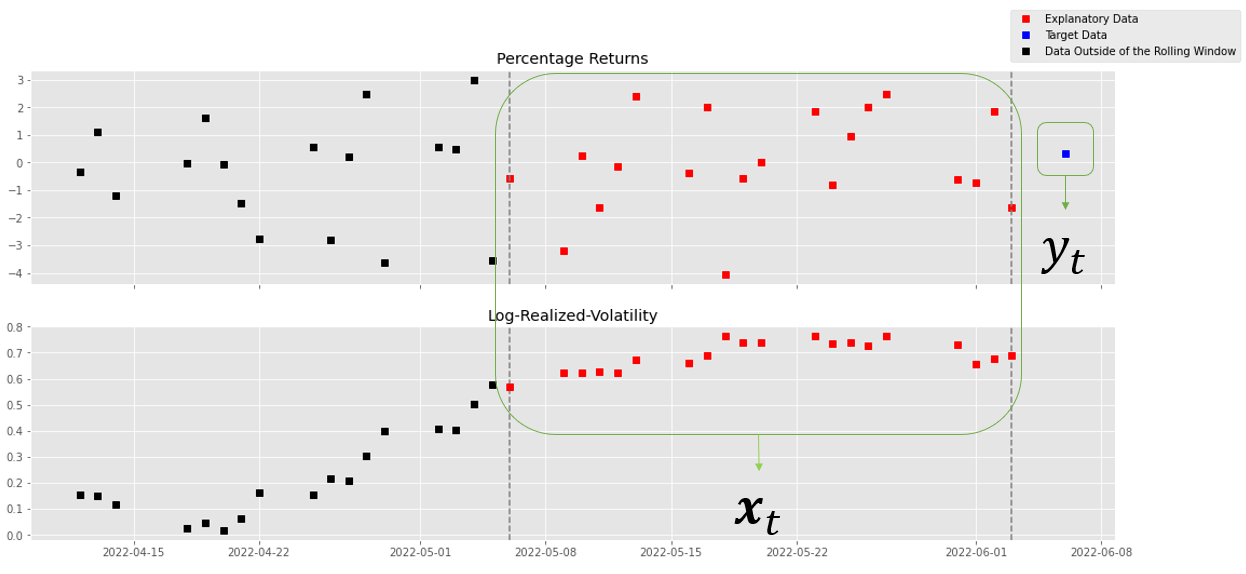
\includegraphics[width = 13cm]{figures/data_variables.png}
     \caption{Data Handling in One Rolling Window}
     \label{fig:data_handl}
 \end{figure}

To what follows, denoting with $\hat{\boldsymbol{\sigma}}(\cdot| \boldsymbol{\theta})$ the outputted volatilities from the parametrized model, we solve the following optimization problem:
\begin{equation}
    \boldsymbol{\theta}^* \coloneqq \underset{\boldsymbol{\theta}}{\mathrm{argmin}}\text{   } l(\mathbf{y}, \hat{\boldsymbol{\sigma}}(\mathbf{X}| \boldsymbol{\theta}))
\end{equation}

with $l(\cdot)$ the loss function defined in \ref{eq:loss1d}.

\begin{mdframed}\begin{remark}\label{rv_discussion}
Equation \ref{eq:rv} is derived from the realized standard deviation of the stocks in rolling windows. The size of the rolling windows is chosen to be 22 which is a popular choice (see \cite{RV_22}) as it is approximately the number of trading days per month. 
\end{remark}\end{mdframed}  

  \begin{mdframed}\begin{remark}\label{ref: lag}
An important hyperparameter of the models is $\lambda$ which determines the \textit{lag} of the returns and log-realized-volatilities taken into consideration. More detailed, at every timestep $t$ we consider a rolling window of the past $\lambda$ days and collect the returns and log-realized-volatilities in this window. The data on every window will be used as explanatory variables to estimate the conditional volatility at the following day. 
\end{remark}\end{mdframed}  


The dataset is consisted of daily returns from 8 famous stock indices covering a time period of approximately 20 years. For a detailed statistical analysis of the data, the reader is referred to \ref{ssec:1d_data} in the Appendix. After a grid search for the lag hyperparameter $\lambda$, we adjust it to 20 in order to balance the computational efficiency and the performance of every model. 

Additionally, for every index the dataset is partitioned into two subsets, namely the \textit{train set} (containing 70\% of the initial dataset) and the \textit{test set} (containing 30\% of the initial dataset). The \textit{train set} is used for parameter estimation or model fitting and the \textit{test set} for performance comparison and evaluation purposes respectively.\todo[]{create remark describing the traintest split} 

\subsection{Definition of the Models}
As baseline statistical models, we select the models GARCH, EGARCH and GJR described in Section \ref{one_d}. In more detail, we estimate the model parameters of the statistical models in the \textit{train set} of every index. The detailed model estimation of these 24 models in total can be reviewed in the Figures \ref{first_8} and \ref{second_8} in the Appendix. 

Regarding the challenger models of this study we developed the models alongside with their tuning to what follows:
\begin{itemize}
    \item \textbf{RNN}:
    A recurrent neural network layer of output size 60 and \textit{tanh} activation function (as introduced in \ref{RNN}) where prior to that, data are passed through a Batch Normalization Layer  (see \ref{BNorm}). The output of the RNN layer is then passed through a dense layer of output size 1 and \textit{exponential} activation function to estimate the conditional volatility of the specific time step. Total number of trainable parameters for the data input described in \ref{data_shape} is 3,849.
    
    \item \textbf{LSTM}:
    A long short term memory layer of output size 60 and \textit{tanh} activation function at the final output (as introduced in \ref{lstm}). Similarly, prior to that data are passed through a Batch Normalization Layer and the output of the LSTM is passed through a Dense Layer of \textit{exponential} activation function. The total number of trainable parameters id 15,189.
    
    \item \textbf{FNN}: 
    A Feed-Forward neural network (as described in \ref{FNN}) of hidden size 300 and output size 1 with activation functions \textit{tanh} and \textit{exponential} respectively. For numerical efficiency, the input of the model was again passed through a Batch Normalization Layer as well.
    
    \item \textbf{GB}:
    A Gradient Tree Boosting estimator as described in \ref{GB}. The number of leaves for the individual small regression trees is fixed to 2, the learning rate $\alpha = .2$ and the number of individual trees $M = 200$. 
    
\end{itemize}


For the fit of the specified models to the data the loss function defined in \ref{eq:loss1d} is used as an objective function for minimization.

The models RNN and LSTM are trained for 10 epochs with a batch size of 2048. For the optimization problem, a Stochastic Gradient Descent variant method was used namely the ADAM algorithm, first introduced by \cite{Adam}. The hyperparameter of the learning rate for the optimizer was adjusted to .008.

FNN model is trained for 20 epochs with a bach size of 1024. Similarly with before, the optimizer selected is ADAM with a fixed learning rate of .001.

Last but not least, for the GB model the Algorithm \ref{gb_alg} is been applied with 2 leaves for every small regression tree, a learning rate $\alpha = .2$ and aggregated over $M=200$ regression trees.

\begin{mdframed}\begin{remark}[Batch Normalization Layer]\label{BNorm}
The specific layer, applies an affine transformation to a given batch of data. In more detail, for a batch of data $\mathfrak{B}$ with sample mean $\mu_{\mathfrak{B}}$ and sample standard deviation $\sigma_{\mathfrak{B}}$, the layer can be seen as function $BN$ where:
\[
\mathfrak{B}\longmapsto BN(\mathfrak{B}| \gamma, \beta) = \gamma\frac{\mathfrak{B}-\mu_\mathfrak{B}}{\sigma_{\mathfrak{B}}}+\beta
\]
where, $\gamma$ and $\beta$ are trainable parameters during the optimization.

The Batch Normalization Layer is mainly used for scaling batches of data close to 0 mean and 1 standard deviation for numerical stability during the backprobagation stage of the training of neural networks and it was first introduced by \cite{BNorm}.
\end{remark}\end{mdframed}

\section{Results \& Comparison}

\subsection{Performance Evaluation}
The performance evaluation of the models is been held with two different approaches.

Firstly, we compare the goodness of fit by following all of the modelling assumptions. In that regard, after optimizing the parameters of the models in the training set, we estimate the conditional volatility for every time step of the test set. Consequently, with the the label vector on the test set $\mathbf{y}_\text{test}$ (containing the realized returns) and the estimated conditional volatility vector $\boldsymbol{\hat{\sigma}}_\text{test}$ (output from the model) we calculate $l(\mathbf{y}_\text{test}, \boldsymbol{\hat{\sigma}}_\text{test})$ where $l$ is defined in \ref{eq:loss1d}. The results from this comparison can be illustrated in Table \ref{nll_results_1d}. 

\begin{mdframed}
\begin{remark}
Note that the loss function described in \ref{eq:loss1d} is not the actual negative log-likelihood of the data. This can be validated if one compares the values of the statistical models in the table \ref{nll_results_1d} and in the Figures \ref{first_8} and \ref{second_8} in the Appendix. This small miss-match occurs from the fact that even that the returns are 0-centered, the MLE estimate for the constant mean $\mu$ is not necessarily 0.

For instance, for the negative log-likelihood of a constant mean - conditionally heteroscedastic model, regarding the score function of $\mu$ one has:
\[\text{nll}(\mathbf{r}| \mu, \boldsymbol{\sigma}) = \frac{1}{2}\left(T\log(2\pi)+\sum_{t} \log(\sigma_t^2) + \left(\frac{r_t-\mu}{\sigma_t}\right)^2\right) \]
\[
\frac{\partial \text{nll}}{\partial \mu} = 0 \Leftrightarrow \mu = \frac{\sum_t r_t/\sigma_t^2}{\sum_t 1/\sigma_t^2}
\]
Although, as already discussed, the selected loss function in \ref{eq:loss1d} is a widely used choice among researchers, in the setup of modelling time varying volatility in financial returns. The mathematical motivation behind it is the conditional martingale assumption of the returns that leads for a 0 constant mean $\mu$. Moreover, due to the small deviation of the daily percentage returns around zero, the modelling dwells on capturing the volatility of the market instead.
\end{remark}
\end{mdframed}

On the contrary to the above loss comparison, we also select another performance evaluation independent with our modelling assumptions. In more detail, we define the \textit{realized volatility} of the data in what follows.



Consequently, we decide to compare the estimated conditional volatility from the models to the realized volatility with the Root Mean Square Error (RMSE) loss function. The results then are evaluated on the \textit{test set} via 

\begin{equation}
    RMSE(\hat{\boldsymbol{\sigma}}_{test}, \mathbf{RV}_{test}) = \left\|\frac{\hat{\boldsymbol{\sigma}}_{test}-\mathbf{RV}_{test}}{\sqrt{N_{test}-22}}\right\|_2
\end{equation}
where, $N_{test}$ denotes the cardinality of the \textit{test set} and $\|\cdot\|$ the Euclidean Norm on $\mathbb{R}^{N_{test}}$.

The specific evaluation selection (given the validity of the \textit{realized volatility} as an index that captures the market's characteristics correctly) captures the model risk of our methodology. Meaning that there is irreducible error due to the Gaussian assumption of the returns and the general modelling approach.

The results of the second comparison can be visualized in Table \ref{RMSE_1d}.
\begin{table}[!ht]
    \centering
    \scriptsize
    \begin{tabular}{|l||l|l|l|l|l|l|l|l|}
    \hline
         \backslashbox{MODEL}{INDEX}& GSPC & DJI & IXIC & RUT & SSMI & OEX & N225 & FTSE \\ \hline\hline
        RNN & 2125 & 2089 & 2532 & 2701 & 2035 & 2166 & 2525 & 2164 \\ \hline
        LSTM & 2082 & 2062 & \textbf{2458} & \textbf{2607} & \textbf{1981} & 2114 & \textbf{2484} & \textbf{2130} \\ \hline
        FNN & 2146 & 2129 & 2865 & 2706 & 2011 & 2156 & 2533 & 2157 \\ \hline
        GB & 2090 & 2069 & 2494 & 2643 & 1999 & 2113 & 2499 & 2163 \\ \hline
        GARCH & 2086 & 2065 & 2487 & 2637 & 2037 & 2110 & 2513 & 2158 \\ \hline
        GJR & \textbf{2075} & \textbf{2049} & 2472 & 2622 & 1998 & \textbf{2106} & 2489 & 2137 \\ \hline
        EGARCH & 2168 & 2141 & 2584 & 2700 & 2111 & 2194 & 2580 & 2217 \\ \hline
    \end{tabular}
    \normalsize
    \caption{Loss Function of the Models in the Test Set}
    \label{nll_results_1d}
\end{table}

\begin{table}[!ht]
    \centering
    \scriptsize
    \begin{tabular}{|l||l|l|l|l|l|l|l|l|}
    \hline
         \backslashbox{MODEL}{INDEX}& GSPC & DJI & IXIC & RUT & SSMI & OEX & N225 & FTSE \\ \hline\hline
        RNN & 0.471 & 0.422 & 0.721 & 0.579 & 0.356 & 0.425 & 0.390 & 0.364 \\ \hline
        LSTM & 0.312 & 0.311 & 0.304 & 0.442 & 0.337 & 0.293 & 0.364 & 0.354 \\ \hline
        FNN & 0.500 & 0.570 & 0.867 & 0.563 & 0.362 & 0.495 & 0.398 & 0.404 \\ \hline
        GB & 0.347 & 0.386 & 0.378 & 0.424 & 0.263 & 0.356 & \textbf{0.235} & 0.241 \\ \hline
        GARCH & \textbf{0.219} & \textbf{0.230} & \textbf{0.207} & \textbf{0.245} & \textbf{0.207} & \textbf{0.220} & 0.241 & \textbf{0.195} \\ \hline
        GJR & 0.301 & 0.310 & 0.275 & 0.334 & 0.263 & 0.300 & 0.294 & 0.281 \\ \hline
        EGARCH & 0.403 & 0.406 & 0.466 & 0.474 & 0.369 & 0.401 & 0.474 & 0.367 \\ \hline
    \end{tabular}
    \normalsize
        \caption{$RMSE$ of the Models}
        \label{RMSE_1d}
\end{table}

\subsection{Comments on the Results}

As can be concluded, regarding the loss comparison the ML models stand out with a marginal difference for most of the indices. From the other hand, when we compare the output with the realized volatility, the statistical GARCH and GJR outperform the ML models.

The main reasoning behind it, is that due to the significantly increased number of the ML models' parameters, the variance of the estimators increases. 



\chapter{Estimation of Models for Multi-Dimensional Returns}


\section{Introduction to Lombard Lending}
\section{Data Handling \& Model Fitting}
\section{Results \& Comparison}
\begin{table}[!ht]
    \scriptsize
    \centering
    \begin{tabular}{|p{3.5cm}||p{1.1cm}|p{1.1cm}|p{1.1cm}|p{1.1cm}|p{1.1cm}|p{1.1cm}|}
    \hline
         & RMSE TRAIN SET & NLL TRAIN SET & RMSE TEST SET & NLL TEST SET & alpha & beta \\ \hline \hline
        Dynamic CC - GARCH & 2.74 & 8983 & 5.09 & -426 & 0.11 & 0.88 \\ \hline
        Constant CC - GARCH & 4.68 & 22860 & 8.12 & 3651 & 0.00 & 0.00 \\ \hline
        Dynamic CC - EGARCH & 2.90 & 8628 & 5.82 & 2562 & 0.11 & 0.89 \\ \hline
        Constant CC - EGARCH & 4.62 & 22647 & 8.66 & 6569 & 0.00 & 0.00 \\ \hline
        Dynamic CC - GJR & 2.76 & 8832 & 5.25 & -663 & 0.11 & 0.89 \\ \hline
        Constant CC - GJR & 4.59 & 22783 & 8.15 & 3462 & 0.00 & 0.00 \\ \hline
        Dynamic CC - GB & 3.05 & 5439 & 9.88 & -2039 & 0.13 & 0.86 \\ \hline
        Constant CC - GB & 4.84 & 21332 & 11.77 & 2133 & 0.00 & 0.00 \\ \hline
        Dynamic CC - FNN & 4.52 & 11774 & 11.90 & 634 & 0.11 & 0.87 \\ \hline
        Constant CC - FNN & 5.61 & 23644 & 13.57 & 2517 & 0.00 & 0.00 \\ \hline
        Dynamic CC - LSTM & 3.37 & 7329 & 7.04 & -1128 & 0.11 & 0.88 \\ \hline
        Constant CC - LSTM & 4.92 & 22256 & 8.91 & 3220 & 0.00 & 0.00 \\ \hline
    \end{tabular}
    \normalsize
    \caption{BH portfolio}
\end{table}

\begin{table}[!ht]
    \centering
    \scriptsize
    \begin{tabular}{|p{3.5cm}||p{1.1cm}|p{1.1cm}|p{1.1cm}|p{1.1cm}|p{1.1cm}|p{1.1cm}|}
    \hline
         & RMSE TRAIN SET & NLL TRAIN SET & RMSE TEST SET & NLL TEST SET & alpha & beta \\ \hline
        Dynamic CC - GARCH & 3.82 & 11602 & 10.75 & 1514 & 0.10 & 0.89 \\ \hline
        Constant CC - GARCH & 5.28 & 20316 & 12.75 & 3903& 0.00 & 0.00 \\ \hline
        Dynamic CC - EGARCH & 4.60 & 12238 & 12.50 & 3628 & 0.14 & 0.78 \\ \hline
        Constant CC - EGARCH & 5.40 & 20235 & 13.91 & 4984 & 0.00 & 0.00 \\ \hline
        Dynamic CC - GJR & 4.69 & 12174 & 12.56 & 2625 & 0.15 & 0.74 \\ \hline
        Constant CC - GJR & 5.30 & 20237 & 13.45 & 3883& 0.00 & 0.00 \\ \hline
        Dynamic CC - GB & 4.39 & 7565 & 17.62 & -455 & 0.15 & 0.84 \\ \hline
        Constant CC - GB & 5.76 & 18829 & 18.58 & 2257 & 0.00 & 0.00 \\ \hline
        Dynamic CC - FNN & 5.21 & 11613 & 17.98 & 2222 & 0.18 & 0.72 \\ \hline
        Constant CC - FNN & 5.74 & 20821 & 18.91 & 3116 & 0.00 & 0.00 \\ \hline
        Dynamic CC - LSTM & 4.85 & 10500 & 13.46 & 1852 & 0.15 & 0.80 \\ \hline
        Constant CC - LSTM & 5.59 & 19812 & 14.77 & 3549 & 0.00 & 0.00 \\ \hline
    \end{tabular}
    \normalsize
    \caption{FTSE}
\end{table}

\begin{table}[!ht]
    \centering
    \scriptsize
    \begin{tabular}{|p{3.5cm}||p{1.1cm}|p{1.1cm}|p{1.1cm}|p{1.1cm}|p{1.1cm}|p{1.1cm}|}
    \hline
         & RMSE TRAIN SET & NLL TRAIN SET & RMSE TEST SET & NLL TEST SET & alpha & beta \\ \hline
        Dynamic CC - GARCH & 3.88 & 4375 & 5.04 & -4603 & 0.12 & 0.87 \\ \hline
        Constant CC - GARCH & 5.73 & 19927 & 6.83 & 11 & 0.00 & 0.00 \\ \hline
        Dynamic CC - EGARCH & 4.60 & 5300 & 7.05 & -738 & 0.13 & 0.83 \\ \hline
        Constant CC - EGARCH & 5.91 & 19947 & 8.17 & 2630 & 0.00 & 0.00 \\ \hline
        Dynamic CC - GJR & 4.09 & 4659 & 6.01 & -4613 & 0.12 & 0.87 \\ \hline
        Constant CC - GJR & 5.69 & 20040 & 7.31 & -4 & 0.00 & 0.00 \\ \hline
        Dynamic CC - GB & 4.58 & 1628 & 7.96 & -5598 & 0.14 & 0.85 \\ \hline
        Constant CC - GB & 6.26 & 18624 & 9.35 & -780 & 0.00 & 0.00 \\ \hline
        Dynamic CC - FNN & 5.31 & 5108 & 9.39 & -4316 & 0.13 & 0.86 \\ \hline
        Constant CC - FNN & 6.78 & 20493 & 10.31 & -160 & 0.00 & 0.00 \\ \hline
        Dynamic CC - LSTM & 4.75 & 3900 & 6.91 & -4791 & 0.12 & 0.87 \\ \hline
        Constant CC - LSTM & 6.18 & 19784 & 8.13 & -73 & 0.00 & 0.00 \\ \hline
    \end{tabular}
    \normalsize
    \caption{SMI}
\end{table}
%--------------------------------------------------------
\chapter{Appendix}
\section{Data}
\subsection{One-Dimensional Data} \label{ssec:1d_data}
The dataset for the analysis of the one dimensional returns was obtained from the \textit{Bloomberg L.P.} software with access from \textit{Zanders Treasury \& Risk}.

We investigated 8 different stock indices with acronyms as follows:
\begin{itemize}
\item GSPC: S\&P 500 INDEX
\item DJI: Dow Jones Industrial Average
\item IXIC: NASDAQ Composite
\item RUT: Russel 2000
\item SSMI: SMI PR
\item OEX: S\&P 100 INDEX
\item N225: NIkkei 225
\item FTSE: FTSE 100
\end{itemize}

The summary statistics of every index alongside with the starting and ending date of investigation are provided in table \ref{tab:summary_1d}.

Admittedly, the values, histograms and autocorrelation plots of the returns can be illustrated in the figures \ref{fig:1d_rets}, \ref{fig:1d_hists} and \ref{fig:1d_auto} respectively.

For most of the returns, the value of the previous day (lag $=$ 1) seems to correlates with the current value and other less significant autocorrelations appear on the 16th previous day (lag $=$ 16). Features that agree with the modelling assumption of conditionally distributed returns.

Moreover, volatility clusters vividly appear on severe periods of the market such us the 2008 crisis and the COVID-19 outbreak. 

Last but not least, the sample distributions of the different indices seem to differ significantly, as fatter tails are observed in IXIC, RUT and N225, fact which contributes to the robustness in the performance of the models.

Regarding the stationarity of the returns we performed the Augmented-Dickey Fuller test \cite{ADF} for each of the series. The resulted test-statistics for every test can be demonstrated in \ref{tb:ADF_table} are significantly smaller than the critical values, concluding to reject the null hypothesis that the time series are non-stationary.

\begin{table}[!ht]\label{tb:ADF_table}
    \scriptsize
    \centering
    \begin{tabular}{|p{1cm}||p{1.cm}|p{1.cm}|p{1.cm}|p{1.cm}|p{1.cm}|p{1.cm}|p{1.cm}|p{1.cm}|}
    \hline
        ~ & GSPC & DJI & IXIC & RUT & SSMI & OEX & N225 & FTSE \\ \hline\hline
        Test Statistic & -14.205 & -14.838 & -13.503 & -13.904 & -13.532 & -14.255 & -12.891 & -14.663 \\ \hline
        p-value & 1.76e-26&	1.85e-27&	2.95e-25&	5.66e-26&	2.61e-25&	1.46e-26&	4.45e-24&	3.36e-27 \\ \hline
        No. lags & 33 & 33 & 33 & 33 & 33 & 33 & 33 & 33 \\ \hline
        No. observations & 5608 & 5608 & 5608 & 5608 & 5595 & 5608 & 5458 & 5629 \\ \hline
        1\% Critical Value & -3.432 & -3.432 & -3.432 & -3.432 & -3.432 & -3.432 & -3.432 & -3.432 \\ \hline
        5\% Critical Value & -2.862 & -2.862 & -2.862 & -2.862 & -2.862 & -2.862 & -2.862 & -2.862 \\ \hline
        10\% Critical Value & -2.567 & -2.567 & -2.567 & -2.567 & -2.567 & -2.567 & -2.567 & -2.567 \\ \hline
    \end{tabular}
    \normalsize	
    \caption{Augmented Dickey–Fuller tests}
\end{table}


\begin{figure}\
    \centering
    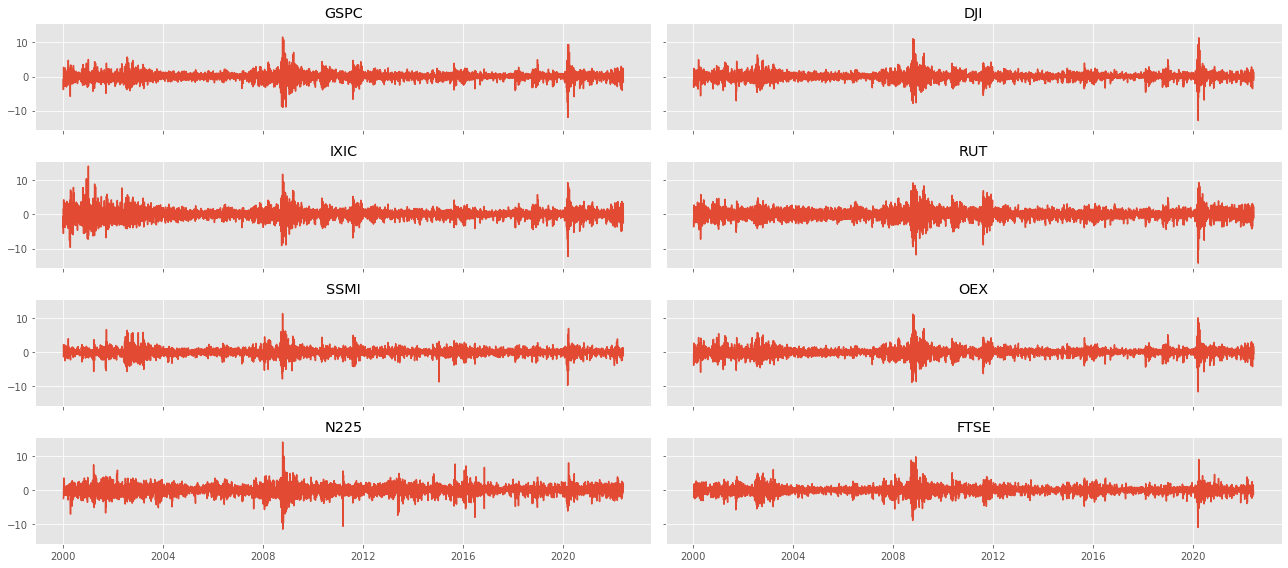
\includegraphics[width = 13cm]{figures/RETURNS.png}
    \caption{Percentage Returns}
    \label{fig:1d_rets}
\end{figure}
\begin{figure}
    \centering
    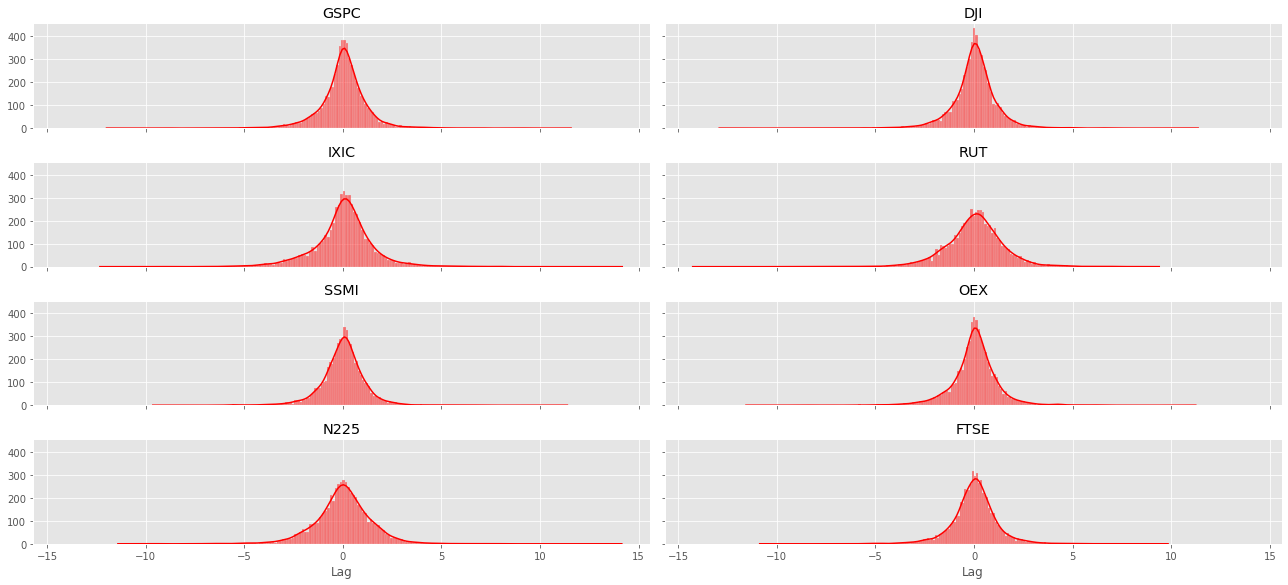
\includegraphics[width = 13cm]{figures/HISTOGRAMMS.png}
    \caption{Histograms of Percentage Returns}
    \label{fig:1d_hists}
\end{figure}
\begin{figure}
    \centering
    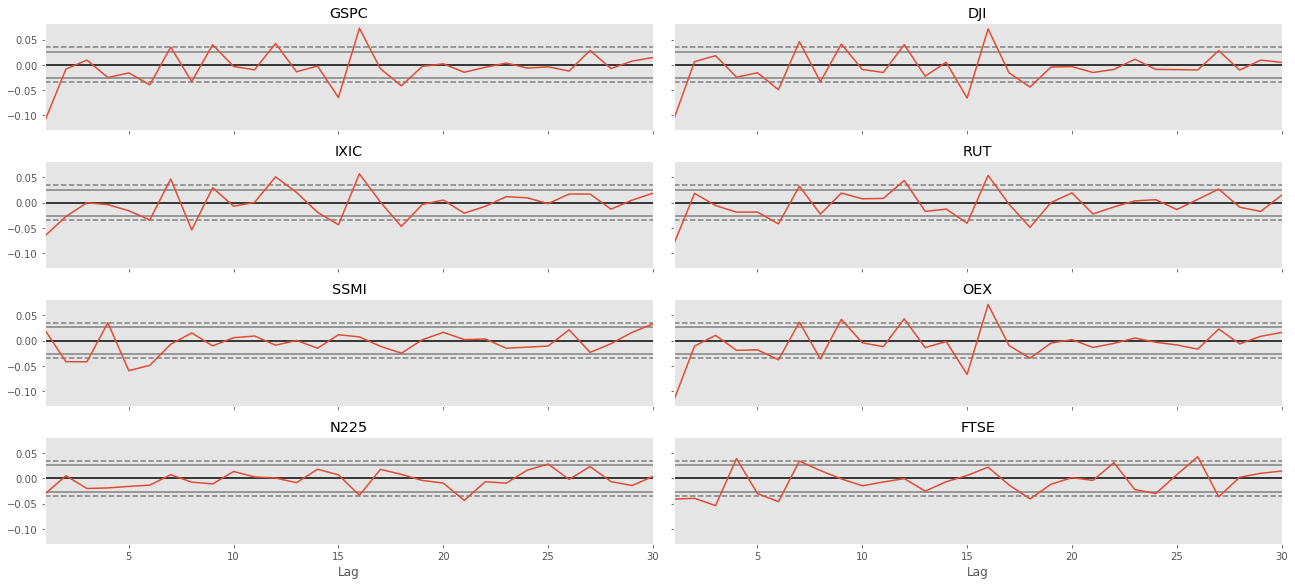
\includegraphics[width = 13cm]{figures/AUTOCORRELATIONS.png}
    \caption{Auto-correlation of Percentage Returns}
    \label{fig:1d_auto}
\end{figure}

\begin{table}[!ht] \label{tab:summary_1d}
    \centering
    \scriptsize
    \begin{tabular}{|p{1.2cm}||p{1.cm}|p{1.cm}|p{1.cm}|p{1.cm}|p{1.cm}|p{1.cm}|p{1.cm}|p{1.cm}|}
    \hline
        ~ & GSPC & DJI & IXIC & RUT & SSMI & OEX & N225 & FTSE \\ \hline\hline
        1st Day & 3/1/00 & 3/1/00 & 3/1/00 & 3/1/00 & 5/1/00 & 3/1/00 & 5/1/00 & 5/1/00 \\ \hline
        Last Day & 3/6/22 & 3/6/22 & 3/6/22 & 3/6/22 & 3/6/22 & 3/6/22 & 3/6/22 & 1/6/22 \\ \hline
        Count & 5642 & 5642 & 5642 & 5642 & 5629 & 5642 & 5491 & 5662 \\ \hline
        Mean & 0.03 & 0.03 & 0.03 & 0.04 & 0.01 & 0.02 & 0.02 & 0.01 \\ \hline
        Std & 1.24 & 1.19 & 1.59 & 1.56 & 1.14 & 1.24 & 1.47 & 1.18 \\ \hline
        Min & -11.98 & -12.93 & -12.32 & -14.27 & -9.64 & -11.57 & -11.41 & -10.87 \\ \hline
        5\%  & -1.90 & -1.80 & -2.60 & -2.39 & -1.76 & -1.90 & -2.30 & -1.83 \\ \hline
        50\%  & 0.06 & 0.05 & 0.09 & 0.08 & 0.05 & 0.06 & 0.04 & 0.05 \\ \hline
        95\%  & 1.74 & 1.68 & 2.33 & 2.33 & 1.65 & 1.76 & 2.20 & 1.76 \\ \hline
        Max & 11.58 & 11.37 & 14.17 & 9.39 & 11.39 & 11.24 & 14.15 & 9.84 \\ \hline
    \end{tabular}
    \normalsize
    \caption{Summary Statistics for the Percentage Returns}
\end{table}

\begin{figure}

\begin{multicols}{2}
{\fontsize{2.5}{4}\selectfont

\begin{center}
\begin{tabular}{lclc}
\toprule
\textbf{Dep. Variable:} &        GSPC        & \textbf{  R-squared:         } &     0.000   \\
\textbf{Mean Model:}    &   Constant Mean    & \textbf{  Adj. R-squared:    } &     0.000   \\
\textbf{Vol Model:}     &       GARCH        & \textbf{  Log-Likelihood:    } &   -5634.73  \\
\textbf{Distribution:}  &       Normal       & \textbf{  AIC:               } &    11277.5  \\
\textbf{Method:}        & Maximum Likelihood & \textbf{  BIC:               } &    11302.6  \\
\textbf{}               &                    & \textbf{  No. Observations:  } &    3949     \\
\textbf{Date:}          &  Mon, Jun 06 2022  & \textbf{  Df Residuals:      } &    3948     \\
\bottomrule
\end{tabular}
\begin{tabular}{lccccc}
            & \textbf{coef} & \textbf{std err} & \textbf{t} & \textbf{P$> |$t$|$} & \textbf{95.0\% Conf. Int.}  \\
\midrule
\textbf{mu} &       0.0356  &    1.351e-02     &     2.637  &      8.369e-03       &   [9.146e-03,6.211e-02]     \\
                  & \textbf{coef} & \textbf{std err} & \textbf{t} & \textbf{P$> |$t$|$} & \textbf{95.0\% Conf. Int.}  \\
\midrule
\textbf{omega}    &       0.0178  &    4.824e-03     &     3.684  &      2.293e-04       &   [8.319e-03,2.723e-02]     \\
\textbf{alpha[1]} &       0.0968  &    1.221e-02     &     7.925  &      2.282e-15       &    [7.283e-02,  0.121]      \\
\textbf{beta[1]}  &       0.8907  &    1.275e-02     &    69.869  &        0.000         &     [  0.866,  0.916]       \\
\bottomrule
\end{tabular}
%\caption{Constant Mean - GARCH Model Results}
\end{center}

  
\begin{center}
\begin{tabular}{lclc}
\toprule
\textbf{Dep. Variable:} &        GSPC        & \textbf{  R-squared:         } &     0.000   \\
\textbf{Mean Model:}    &   Constant Mean    & \textbf{  Adj. R-squared:    } &     0.000   \\
\textbf{Vol Model:}     &     GJR-GARCH      & \textbf{  Log-Likelihood:    } &   -5538.65  \\
\textbf{Distribution:}  &       Normal       & \textbf{  AIC:               } &    11087.3  \\
\textbf{Method:}        & Maximum Likelihood & \textbf{  BIC:               } &    11118.7  \\
\textbf{}               &                    & \textbf{  No. Observations:  } &    3949     \\
\textbf{Date:}          &  Mon, Jun 06 2022  & \textbf{  Df Residuals:      } &    3948     \\
\bottomrule
\end{tabular}
\begin{tabular}{lccccc}
            & \textbf{coef} & \textbf{std err} & \textbf{t} & \textbf{P$> |$t$|$} & \textbf{95.0\% Conf. Int.}  \\
\midrule
\textbf{mu} &  -7.1443e-03  &    1.389e-02     &    -0.514  &          0.607       &   [-3.437e-02,2.008e-02]    \\
                  & \textbf{coef} & \textbf{std err} & \textbf{t} & \textbf{P$> |$t$|$} & \textbf{95.0\% Conf. Int.}  \\
\midrule
\textbf{omega}    &       0.0190  &    4.450e-03     &     4.278  &      1.887e-05       &   [1.031e-02,2.776e-02]     \\
\textbf{alpha[1]} &   2.5982e-10  &    1.225e-02     & 2.122e-08  &          1.000       &   [-2.400e-02,2.400e-02]    \\
\textbf{gamma[1]} &       0.1731  &    2.175e-02     &     7.958  &      1.743e-15       &     [  0.130,  0.216]       \\
\textbf{beta[1]}  &       0.8987  &    1.619e-02     &    55.493  &        0.000         &     [  0.867,  0.930]       \\
\bottomrule
\end{tabular}
%\caption{Constant Mean - GJR-GARCH Model Results}
\end{center}

  
\begin{center}
\begin{tabular}{lclc}
\toprule
\textbf{Dep. Variable:} &        GSPC        & \textbf{  R-squared:         } &     0.000   \\
\textbf{Mean Model:}    &   Constant Mean    & \textbf{  Adj. R-squared:    } &     0.000   \\
\textbf{Vol Model:}     &       EGARCH       & \textbf{  Log-Likelihood:    } &   -5535.30  \\
\textbf{Distribution:}  &       Normal       & \textbf{  AIC:               } &    11080.6  \\
\textbf{Method:}        & Maximum Likelihood & \textbf{  BIC:               } &    11112.0  \\
\textbf{}               &                    & \textbf{  No. Observations:  } &    3949     \\
\textbf{Date:}          &  Mon, Jun 06 2022  & \textbf{  Df Residuals:      } &    3948     \\
\bottomrule
\end{tabular}
\begin{tabular}{lccccc}
            & \textbf{coef} & \textbf{std err} & \textbf{t} & \textbf{P$> |$t$|$} & \textbf{95.0\% Conf. Int.}  \\
\midrule
\textbf{mu} &  -6.0538e-03  &    1.333e-02     &    -0.454  &          0.650       &   [-3.218e-02,2.007e-02]    \\
                  & \textbf{coef} & \textbf{std err} & \textbf{t} & \textbf{P$> |$t$|$} & \textbf{95.0\% Conf. Int.}  \\
\midrule
\textbf{omega}    &   2.2315e-03  &    3.045e-03     &     0.733  &          0.464       &   [-3.736e-03,8.199e-03]    \\
\textbf{alpha[1]} &       0.1159  &    1.600e-02     &     7.244  &      4.359e-13       &    [8.454e-02,  0.147]      \\
\textbf{gamma[1]} &      -0.1478  &    1.491e-02     &    -9.911  &      3.740e-23       &     [ -0.177, -0.119]       \\
\textbf{beta[1]}  &       0.9793  &    4.376e-03     &   223.780  &        0.000         &     [  0.971,  0.988]       \\
\bottomrule
\end{tabular}
%\caption{Constant Mean - EGARCH Model Results}
\end{center}

  
\begin{center}
\begin{tabular}{lclc}
\toprule
\textbf{Dep. Variable:} &         DJI        & \textbf{  R-squared:         } &     0.000   \\
\textbf{Mean Model:}    &   Constant Mean    & \textbf{  Adj. R-squared:    } &     0.000   \\
\textbf{Vol Model:}     &       GARCH        & \textbf{  Log-Likelihood:    } &   -5415.23  \\
\textbf{Distribution:}  &       Normal       & \textbf{  AIC:               } &    10838.5  \\
\textbf{Method:}        & Maximum Likelihood & \textbf{  BIC:               } &    10863.6  \\
\textbf{}               &                    & \textbf{  No. Observations:  } &    3949     \\
\textbf{Date:}          &  Mon, Jun 06 2022  & \textbf{  Df Residuals:      } &    3948     \\
\bottomrule
\end{tabular}
\begin{tabular}{lccccc}
            & \textbf{coef} & \textbf{std err} & \textbf{t} & \textbf{P$> |$t$|$} & \textbf{95.0\% Conf. Int.}  \\
\midrule
\textbf{mu} &       0.0353  &    1.289e-02     &     2.741  &      6.121e-03       &   [1.007e-02,6.061e-02]     \\
                  & \textbf{coef} & \textbf{std err} & \textbf{t} & \textbf{P$> |$t$|$} & \textbf{95.0\% Conf. Int.}  \\
\midrule
\textbf{omega}    &       0.0168  &    4.380e-03     &     3.841  &      1.227e-04       &   [8.238e-03,2.541e-02]     \\
\textbf{alpha[1]} &       0.1028  &    1.328e-02     &     7.741  &      9.882e-15       &    [7.679e-02,  0.129]      \\
\textbf{beta[1]}  &       0.8847  &    1.326e-02     &    66.717  &        0.000         &     [  0.859,  0.911]       \\
\bottomrule
\end{tabular}
%\caption{Constant Mean - GARCH Model Results}
\end{center}

  
\begin{center}
\begin{tabular}{lclc}
\toprule
\textbf{Dep. Variable:} &         DJI        & \textbf{  R-squared:         } &     0.000   \\
\textbf{Mean Model:}    &   Constant Mean    & \textbf{  Adj. R-squared:    } &     0.000   \\
\textbf{Vol Model:}     &     GJR-GARCH      & \textbf{  Log-Likelihood:    } &   -5326.13  \\
\textbf{Distribution:}  &       Normal       & \textbf{  AIC:               } &    10662.3  \\
\textbf{Method:}        & Maximum Likelihood & \textbf{  BIC:               } &    10693.7  \\
\textbf{}               &                    & \textbf{  No. Observations:  } &    3949     \\
\textbf{Date:}          &  Mon, Jun 06 2022  & \textbf{  Df Residuals:      } &    3948     \\
\bottomrule
\end{tabular}
\begin{tabular}{lccccc}
            & \textbf{coef} & \textbf{std err} & \textbf{t} & \textbf{P$> |$t$|$} & \textbf{95.0\% Conf. Int.}  \\
\midrule
\textbf{mu} &  -4.2380e-03  &    1.301e-02     &    -0.326  &          0.745       &   [-2.975e-02,2.127e-02]    \\
                  & \textbf{coef} & \textbf{std err} & \textbf{t} & \textbf{P$> |$t$|$} & \textbf{95.0\% Conf. Int.}  \\
\midrule
\textbf{omega}    &       0.0164  &    3.735e-03     &     4.384  &      1.163e-05       &   [9.055e-03,2.369e-02]     \\
\textbf{alpha[1]} &   1.8615e-09  &    1.062e-02     & 1.753e-07  &          1.000       &   [-2.081e-02,2.081e-02]    \\
\textbf{gamma[1]} &       0.1756  &    2.299e-02     &     7.640  &      2.164e-14       &     [  0.131,  0.221]       \\
\textbf{beta[1]}  &       0.8993  &    1.469e-02     &    61.237  &        0.000         &     [  0.870,  0.928]       \\
\bottomrule
\end{tabular}
%\caption{Constant Mean - GJR-GARCH Model Results}
\end{center}

  
\begin{center}
\begin{tabular}{lclc}
\toprule
\textbf{Dep. Variable:} &         DJI        & \textbf{  R-squared:         } &     0.000   \\
\textbf{Mean Model:}    &   Constant Mean    & \textbf{  Adj. R-squared:    } &     0.000   \\
\textbf{Vol Model:}     &       EGARCH       & \textbf{  Log-Likelihood:    } &   -5322.12  \\
\textbf{Distribution:}  &       Normal       & \textbf{  AIC:               } &    10654.2  \\
\textbf{Method:}        & Maximum Likelihood & \textbf{  BIC:               } &    10685.6  \\
\textbf{}               &                    & \textbf{  No. Observations:  } &    3949     \\
\textbf{Date:}          &  Mon, Jun 06 2022  & \textbf{  Df Residuals:      } &    3948     \\
\bottomrule
\end{tabular}
\begin{tabular}{lccccc}
            & \textbf{coef} & \textbf{std err} & \textbf{t} & \textbf{P$> |$t$|$} & \textbf{95.0\% Conf. Int.}  \\
\midrule
\textbf{mu} &  -4.9676e-03  &    1.260e-02     &    -0.394  &          0.693       &   [-2.967e-02,1.973e-02]    \\
                  & \textbf{coef} & \textbf{std err} & \textbf{t} & \textbf{P$> |$t$|$} & \textbf{95.0\% Conf. Int.}  \\
\midrule
\textbf{omega}    &   4.3778e-04  &    2.899e-03     &     0.151  &          0.880       &   [-5.244e-03,6.119e-03]    \\
\textbf{alpha[1]} &       0.1247  &    1.717e-02     &     7.264  &      3.765e-13       &    [9.107e-02,  0.158]      \\
\textbf{gamma[1]} &      -0.1421  &    1.464e-02     &    -9.707  &      2.823e-22       &     [ -0.171, -0.113]       \\
\textbf{beta[1]}  &       0.9791  &    4.254e-03     &   230.143  &        0.000         &     [  0.971,  0.987]       \\
\bottomrule
\end{tabular}
%\caption{Constant Mean - EGARCH Model Results}
\end{center}

  
\begin{center}
\begin{tabular}{lclc}
\toprule
\textbf{Dep. Variable:} &        IXIC        & \textbf{  R-squared:         } &     0.000   \\
\textbf{Mean Model:}    &   Constant Mean    & \textbf{  Adj. R-squared:    } &     0.000   \\
\textbf{Vol Model:}     &       GARCH        & \textbf{  Log-Likelihood:    } &   -6658.56  \\
\textbf{Distribution:}  &       Normal       & \textbf{  AIC:               } &    13325.1  \\
\textbf{Method:}        & Maximum Likelihood & \textbf{  BIC:               } &    13350.2  \\
\textbf{}               &                    & \textbf{  No. Observations:  } &    3949     \\
\textbf{Date:}          &  Mon, Jun 06 2022  & \textbf{  Df Residuals:      } &    3948     \\
\bottomrule
\end{tabular}
\begin{tabular}{lccccc}
            & \textbf{coef} & \textbf{std err} & \textbf{t} & \textbf{P$> |$t$|$} & \textbf{95.0\% Conf. Int.}  \\
\midrule
\textbf{mu} &       0.0526  &    1.751e-02     &     3.006  &      2.648e-03       &   [1.831e-02,8.694e-02]     \\
                  & \textbf{coef} & \textbf{std err} & \textbf{t} & \textbf{P$> |$t$|$} & \textbf{95.0\% Conf. Int.}  \\
\midrule
\textbf{omega}    &       0.0185  &    4.759e-03     &     3.886  &      1.020e-04       &   [9.165e-03,2.782e-02]     \\
\textbf{alpha[1]} &       0.0828  &    1.060e-02     &     7.814  &      5.559e-15       &    [6.205e-02,  0.104]      \\
\textbf{beta[1]}  &       0.9091  &    1.062e-02     &    85.602  &        0.000         &     [  0.888,  0.930]       \\
\bottomrule
\end{tabular}
%\caption{Constant Mean - GARCH Model Results}
\end{center}

  
\begin{center}
\begin{tabular}{lclc}
\toprule
\textbf{Dep. Variable:} &        IXIC        & \textbf{  R-squared:         } &     0.000   \\
\textbf{Mean Model:}    &   Constant Mean    & \textbf{  Adj. R-squared:    } &     0.000   \\
\textbf{Vol Model:}     &     GJR-GARCH      & \textbf{  Log-Likelihood:    } &   -6593.88  \\
\textbf{Distribution:}  &       Normal       & \textbf{  AIC:               } &    13197.8  \\
\textbf{Method:}        & Maximum Likelihood & \textbf{  BIC:               } &    13229.2  \\
\textbf{}               &                    & \textbf{  No. Observations:  } &    3949     \\
\textbf{Date:}          &  Mon, Jun 06 2022  & \textbf{  Df Residuals:      } &    3948     \\
\bottomrule
\end{tabular}
\begin{tabular}{lccccc}
            & \textbf{coef} & \textbf{std err} & \textbf{t} & \textbf{P$> |$t$|$} & \textbf{95.0\% Conf. Int.}  \\
\midrule
\textbf{mu} &   8.6125e-03  &    1.721e-02     &     0.500  &          0.617       &   [-2.512e-02,4.235e-02]    \\
                  & \textbf{coef} & \textbf{std err} & \textbf{t} & \textbf{P$> |$t$|$} & \textbf{95.0\% Conf. Int.}  \\
\midrule
\textbf{omega}    &       0.0191  &    4.967e-03     &     3.855  &      1.158e-04       &   [9.411e-03,2.888e-02]     \\
\textbf{alpha[1]} &   4.1946e-17  &    7.526e-03     & 5.574e-15  &          1.000       &   [-1.475e-02,1.475e-02]    \\
\textbf{gamma[1]} &       0.1340  &    1.816e-02     &     7.378  &      1.606e-13       &    [9.842e-02,  0.170]      \\
\textbf{beta[1]}  &       0.9228  &    1.231e-02     &    74.985  &        0.000         &     [  0.899,  0.947]       \\
\bottomrule
\end{tabular}
%\caption{Constant Mean - GJR-GARCH Model Results}
\end{center}

  
\begin{center}
\begin{tabular}{lclc}
\toprule
\textbf{Dep. Variable:} &        IXIC        & \textbf{  R-squared:         } &     0.000   \\
\textbf{Mean Model:}    &   Constant Mean    & \textbf{  Adj. R-squared:    } &     0.000   \\
\textbf{Vol Model:}     &       EGARCH       & \textbf{  Log-Likelihood:    } &   -6591.56  \\
\textbf{Distribution:}  &       Normal       & \textbf{  AIC:               } &    13193.1  \\
\textbf{Method:}        & Maximum Likelihood & \textbf{  BIC:               } &    13224.5  \\
\textbf{}               &                    & \textbf{  No. Observations:  } &    3949     \\
\textbf{Date:}          &  Mon, Jun 06 2022  & \textbf{  Df Residuals:      } &    3948     \\
\bottomrule
\end{tabular}
\begin{tabular}{lccccc}
            & \textbf{coef} & \textbf{std err} & \textbf{t} & \textbf{P$> |$t$|$} & \textbf{95.0\% Conf. Int.}  \\
\midrule
\textbf{mu} &   4.6614e-03  &    1.705e-02     &     0.273  &          0.785       &   [-2.876e-02,3.809e-02]    \\
                  & \textbf{coef} & \textbf{std err} & \textbf{t} & \textbf{P$> |$t$|$} & \textbf{95.0\% Conf. Int.}  \\
\midrule
\textbf{omega}    &   8.6029e-03  &    3.203e-03     &     2.686  &      7.231e-03       &   [2.325e-03,1.488e-02]     \\
\textbf{alpha[1]} &       0.1099  &    1.642e-02     &     6.693  &      2.187e-11       &    [7.774e-02,  0.142]      \\
\textbf{gamma[1]} &      -0.1062  &    1.097e-02     &    -9.675  &      3.846e-22       &    [ -0.128,-8.465e-02]     \\
\textbf{beta[1]}  &       0.9863  &    2.852e-03     &   345.832  &        0.000         &     [  0.981,  0.992]       \\
\bottomrule
\end{tabular}
%\caption{Constant Mean - EGARCH Model Results}
\end{center}

  
\begin{center}
\begin{tabular}{lclc}
\toprule
\textbf{Dep. Variable:} &         RUT        & \textbf{  R-squared:         } &     0.000   \\
\textbf{Mean Model:}    &   Constant Mean    & \textbf{  Adj. R-squared:    } &     0.000   \\
\textbf{Vol Model:}     &       GARCH        & \textbf{  Log-Likelihood:    } &   -6743.16  \\
\textbf{Distribution:}  &       Normal       & \textbf{  AIC:               } &    13494.3  \\
\textbf{Method:}        & Maximum Likelihood & \textbf{  BIC:               } &    13519.4  \\
\textbf{}               &                    & \textbf{  No. Observations:  } &    3949     \\
\textbf{Date:}          &  Mon, Jun 06 2022  & \textbf{  Df Residuals:      } &    3948     \\
\bottomrule
\end{tabular}
\begin{tabular}{lccccc}
            & \textbf{coef} & \textbf{std err} & \textbf{t} & \textbf{P$> |$t$|$} & \textbf{95.0\% Conf. Int.}  \\
\midrule
\textbf{mu} &       0.0337  &    1.883e-02     &     1.788  &      7.380e-02       &   [-3.241e-03,7.057e-02]    \\
                  & \textbf{coef} & \textbf{std err} & \textbf{t} & \textbf{P$> |$t$|$} & \textbf{95.0\% Conf. Int.}  \\
\midrule
\textbf{omega}    &       0.0398  &    9.273e-03     &     4.293  &      1.760e-05       &   [2.164e-02,5.798e-02]     \\
\textbf{alpha[1]} &       0.0870  &    1.101e-02     &     7.904  &      2.697e-15       &    [6.546e-02,  0.109]      \\
\textbf{beta[1]}  &       0.8932  &    1.289e-02     &    69.302  &        0.000         &     [  0.868,  0.918]       \\
\bottomrule
\end{tabular}
%\caption{Constant Mean - GARCH Model Results}
\end{center}

  
\begin{center}
\begin{tabular}{lclc}
\toprule
\textbf{Dep. Variable:} &         RUT        & \textbf{  R-squared:         } &     0.000   \\
\textbf{Mean Model:}    &   Constant Mean    & \textbf{  Adj. R-squared:    } &     0.000   \\
\textbf{Vol Model:}     &     GJR-GARCH      & \textbf{  Log-Likelihood:    } &   -6686.91  \\
\textbf{Distribution:}  &       Normal       & \textbf{  AIC:               } &    13383.8  \\
\textbf{Method:}        & Maximum Likelihood & \textbf{  BIC:               } &    13415.2  \\
\textbf{}               &                    & \textbf{  No. Observations:  } &    3949     \\
\textbf{Date:}          &  Mon, Jun 06 2022  & \textbf{  Df Residuals:      } &    3948     \\
\bottomrule
\end{tabular}
\begin{tabular}{lccccc}
            & \textbf{coef} & \textbf{std err} & \textbf{t} & \textbf{P$> |$t$|$} & \textbf{95.0\% Conf. Int.}  \\
\midrule
\textbf{mu} &      -0.0143  &    1.912e-02     &    -0.748  &          0.455       &   [-5.177e-02,2.318e-02]    \\
                  & \textbf{coef} & \textbf{std err} & \textbf{t} & \textbf{P$> |$t$|$} & \textbf{95.0\% Conf. Int.}  \\
\midrule
\textbf{omega}    &       0.0415  &    9.592e-03     &     4.324  &      1.530e-05       &   [2.268e-02,6.028e-02]     \\
\textbf{alpha[1]} &     0.0000    &    7.306e-03     &   0.000    &          1.000       &   [-1.432e-02,1.432e-02]    \\
\textbf{gamma[1]} &       0.1436  &    2.046e-02     &     7.018  &      2.251e-12       &     [  0.104,  0.184]       \\
\textbf{beta[1]}  &       0.9069  &    1.348e-02     &    67.288  &        0.000         &     [  0.880,  0.933]       \\
\bottomrule
\end{tabular}
%\caption{Constant Mean - GJR-GARCH Model Results}
\end{center}

  
\begin{center}
\begin{tabular}{lclc}
\toprule
\textbf{Dep. Variable:} &         RUT        & \textbf{  R-squared:         } &     0.000   \\
\textbf{Mean Model:}    &   Constant Mean    & \textbf{  Adj. R-squared:    } &     0.000   \\
\textbf{Vol Model:}     &       EGARCH       & \textbf{  Log-Likelihood:    } &   -6690.03  \\
\textbf{Distribution:}  &       Normal       & \textbf{  AIC:               } &    13390.1  \\
\textbf{Method:}        & Maximum Likelihood & \textbf{  BIC:               } &    13421.5  \\
\textbf{}               &                    & \textbf{  No. Observations:  } &    3949     \\
\textbf{Date:}          &  Mon, Jun 06 2022  & \textbf{  Df Residuals:      } &    3948     \\
\bottomrule
\end{tabular}
\begin{tabular}{lccccc}
            & \textbf{coef} & \textbf{std err} & \textbf{t} & \textbf{P$> |$t$|$} & \textbf{95.0\% Conf. Int.}  \\
\midrule
\textbf{mu} &      -0.0197  &    1.894e-02     &    -1.039  &          0.299       &   [-5.681e-02,1.743e-02]    \\
                  & \textbf{coef} & \textbf{std err} & \textbf{t} & \textbf{P$> |$t$|$} & \textbf{95.0\% Conf. Int.}  \\
\midrule
\textbf{omega}    &       0.0135  &    4.078e-03     &     3.313  &      9.231e-04       &   [5.518e-03,2.150e-02]     \\
\textbf{alpha[1]} &       0.1247  &    1.421e-02     &     8.772  &      1.757e-18       &    [9.681e-02,  0.153]      \\
\textbf{gamma[1]} &      -0.1104  &    1.237e-02     &    -8.921  &      4.601e-19       &    [ -0.135,-8.612e-02]     \\
\textbf{beta[1]}  &       0.9779  &    4.507e-03     &   216.972  &        0.000         &     [  0.969,  0.987]       \\
\bottomrule
\end{tabular}
%\caption{Constant Mean - EGARCH Model Results}
\end{center}
}
\end{multicols}
\caption{GSPC, DJI, IXIC, RUT Arch Models}
\label{first_8}
\end{figure}


\begin{figure}

\begin{multicols}{2}
{\fontsize{2.5}{4}\selectfont
  
\begin{center}
\begin{tabular}{lclc}
\toprule
\textbf{Dep. Variable:} &        SSMI        & \textbf{  R-squared:         } &     0.000   \\
\textbf{Mean Model:}    &   Constant Mean    & \textbf{  Adj. R-squared:    } &     0.000   \\
\textbf{Vol Model:}     &       GARCH        & \textbf{  Log-Likelihood:    } &   -5536.80  \\
\textbf{Distribution:}  &       Normal       & \textbf{  AIC:               } &    11081.6  \\
\textbf{Method:}        & Maximum Likelihood & \textbf{  BIC:               } &    11106.7  \\
\textbf{}               &                    & \textbf{  No. Observations:  } &    3940     \\
\textbf{Date:}          &  Mon, Jun 06 2022  & \textbf{  Df Residuals:      } &    3939     \\
\bottomrule
\end{tabular}
\begin{tabular}{lccccc}
            & \textbf{coef} & \textbf{std err} & \textbf{t} & \textbf{P$> |$t$|$} & \textbf{95.0\% Conf. Int.}  \\
\midrule
\textbf{mu} &       0.0415  &    1.368e-02     &     3.032  &      2.429e-03       &   [1.466e-02,6.828e-02]     \\
                  & \textbf{coef} & \textbf{std err} & \textbf{t} & \textbf{P$> |$t$|$} & \textbf{95.0\% Conf. Int.}  \\
\midrule
\textbf{omega}    &       0.0283  &    6.045e-03     &     4.681  &      2.861e-06       &   [1.645e-02,4.014e-02]     \\
\textbf{alpha[1]} &       0.1276  &    1.506e-02     &     8.476  &      2.326e-17       &    [9.812e-02,  0.157]      \\
\textbf{beta[1]}  &       0.8534  &    1.484e-02     &    57.503  &        0.000         &     [  0.824,  0.882]       \\
\bottomrule
\end{tabular}
%\caption{Constant Mean - GARCH Model Results}
\end{center}

\begin{center}
\begin{tabular}{lclc}
\toprule
\textbf{Dep. Variable:} &        SSMI        & \textbf{  R-squared:         } &     0.000   \\
\textbf{Mean Model:}    &   Constant Mean    & \textbf{  Adj. R-squared:    } &     0.000   \\
\textbf{Vol Model:}     &     GJR-GARCH      & \textbf{  Log-Likelihood:    } &   -5467.91  \\
\textbf{Distribution:}  &       Normal       & \textbf{  AIC:               } &    10945.8  \\
\textbf{Method:}        & Maximum Likelihood & \textbf{  BIC:               } &    10977.2  \\
\textbf{}               &                    & \textbf{  No. Observations:  } &    3940     \\
\textbf{Date:}          &  Mon, Jun 06 2022  & \textbf{  Df Residuals:      } &    3939     \\
\bottomrule
\end{tabular}
\begin{tabular}{lccccc}
            & \textbf{coef} & \textbf{std err} & \textbf{t} & \textbf{P$> |$t$|$} & \textbf{95.0\% Conf. Int.}  \\
\midrule
\textbf{mu} &   5.3048e-03  &    1.318e-02     &     0.402  &          0.687       &   [-2.053e-02,3.114e-02]    \\
                  & \textbf{coef} & \textbf{std err} & \textbf{t} & \textbf{P$> |$t$|$} & \textbf{95.0\% Conf. Int.}  \\
\midrule
\textbf{omega}    &       0.0269  &    5.124e-03     &     5.248  &      1.537e-07       &   [1.685e-02,3.694e-02]     \\
\textbf{alpha[1]} &       0.0155  &    1.846e-02     &     0.840  &          0.401       &   [-2.068e-02,5.168e-02]    \\
\textbf{gamma[1]} &       0.1768  &    2.422e-02     &     7.299  &      2.906e-13       &     [  0.129,  0.224]       \\
\textbf{beta[1]}  &       0.8749  &    1.496e-02     &    58.500  &        0.000         &     [  0.846,  0.904]       \\
\bottomrule
\end{tabular}
%\caption{Constant Mean - GJR-GARCH Model Results}
\end{center}

  
\begin{center}
\begin{tabular}{lclc}
\toprule
\textbf{Dep. Variable:} &        SSMI        & \textbf{  R-squared:         } &     0.000   \\
\textbf{Mean Model:}    &   Constant Mean    & \textbf{  Adj. R-squared:    } &     0.000   \\
\textbf{Vol Model:}     &       EGARCH       & \textbf{  Log-Likelihood:    } &   -5446.28  \\
\textbf{Distribution:}  &       Normal       & \textbf{  AIC:               } &    10902.6  \\
\textbf{Method:}        & Maximum Likelihood & \textbf{  BIC:               } &    10934.0  \\
\textbf{}               &                    & \textbf{  No. Observations:  } &    3940     \\
\textbf{Date:}          &  Mon, Jun 06 2022  & \textbf{  Df Residuals:      } &    3939     \\
\bottomrule
\end{tabular}
\begin{tabular}{lccccc}
            & \textbf{coef} & \textbf{std err} & \textbf{t} & \textbf{P$> |$t$|$} & \textbf{95.0\% Conf. Int.}  \\
\midrule
\textbf{mu} &  -7.9094e-04  &    3.514e-03     &    -0.225  &          0.822       &   [-7.679e-03,6.097e-03]    \\
                  & \textbf{coef} & \textbf{std err} & \textbf{t} & \textbf{P$> |$t$|$} & \textbf{95.0\% Conf. Int.}  \\
\midrule
\textbf{omega}    &   1.6752e-03  &    3.175e-03     &     0.528  &          0.598       &   [-4.549e-03,7.899e-03]    \\
\textbf{alpha[1]} &       0.1501  &    2.216e-02     &     6.774  &      1.249e-11       &     [  0.107,  0.194]       \\
\textbf{gamma[1]} &      -0.1388  &    1.256e-02     &   -11.052  &      2.148e-28       &     [ -0.163, -0.114]       \\
\textbf{beta[1]}  &       0.9733  &    3.940e-03     &   247.002  &        0.000         &     [  0.966,  0.981]       \\
\bottomrule
\end{tabular}
%\caption{Constant Mean - EGARCH Model Results}
\end{center}

  
\begin{center}
\begin{tabular}{lclc}
\toprule
\textbf{Dep. Variable:} &         OEX        & \textbf{  R-squared:         } &     0.000   \\
\textbf{Mean Model:}    &   Constant Mean    & \textbf{  Adj. R-squared:    } &     0.000   \\
\textbf{Vol Model:}     &       GARCH        & \textbf{  Log-Likelihood:    } &   -5607.86  \\
\textbf{Distribution:}  &       Normal       & \textbf{  AIC:               } &    11223.7  \\
\textbf{Method:}        & Maximum Likelihood & \textbf{  BIC:               } &    11248.8  \\
\textbf{}               &                    & \textbf{  No. Observations:  } &    3949     \\
\textbf{Date:}          &  Mon, Jun 06 2022  & \textbf{  Df Residuals:      } &    3948     \\
\bottomrule
\end{tabular}
\begin{tabular}{lccccc}
            & \textbf{coef} & \textbf{std err} & \textbf{t} & \textbf{P$> |$t$|$} & \textbf{95.0\% Conf. Int.}  \\
\midrule
\textbf{mu} &       0.0391  &    1.332e-02     &     2.931  &      3.382e-03       &   [1.294e-02,6.517e-02]     \\
                  & \textbf{coef} & \textbf{std err} & \textbf{t} & \textbf{P$> |$t$|$} & \textbf{95.0\% Conf. Int.}  \\
\midrule
\textbf{omega}    &       0.0171  &    4.802e-03     &     3.564  &      3.658e-04       &   [7.702e-03,2.653e-02]     \\
\textbf{alpha[1]} &       0.1007  &    1.303e-02     &     7.732  &      1.060e-14       &    [7.518e-02,  0.126]      \\
\textbf{beta[1]}  &       0.8878  &    1.339e-02     &    66.323  &        0.000         &     [  0.862,  0.914]       \\
\bottomrule
\end{tabular}
%\caption{Constant Mean - GARCH Model Results}
\end{center}

  
\begin{center}
\begin{tabular}{lclc}
\toprule
\textbf{Dep. Variable:} &         OEX        & \textbf{  R-squared:         } &     0.000   \\
\textbf{Mean Model:}    &   Constant Mean    & \textbf{  Adj. R-squared:    } &     0.000   \\
\textbf{Vol Model:}     &     GJR-GARCH      & \textbf{  Log-Likelihood:    } &   -5511.65  \\
\textbf{Distribution:}  &       Normal       & \textbf{  AIC:               } &    11033.3  \\
\textbf{Method:}        & Maximum Likelihood & \textbf{  BIC:               } &    11064.7  \\
\textbf{}               &                    & \textbf{  No. Observations:  } &    3949     \\
\textbf{Date:}          &  Mon, Jun 06 2022  & \textbf{  Df Residuals:      } &    3948     \\
\bottomrule
\end{tabular}
\begin{tabular}{lccccc}
            & \textbf{coef} & \textbf{std err} & \textbf{t} & \textbf{P$> |$t$|$} & \textbf{95.0\% Conf. Int.}  \\
\midrule
\textbf{mu} &  -2.0264e-03  &    1.350e-02     &    -0.150  &          0.881       &   [-2.848e-02,2.443e-02]    \\
                  & \textbf{coef} & \textbf{std err} & \textbf{t} & \textbf{P$> |$t$|$} & \textbf{95.0\% Conf. Int.}  \\
\midrule
\textbf{omega}    &       0.0181  &    4.150e-03     &     4.357  &      1.321e-05       &   [9.947e-03,2.622e-02]     \\
\textbf{alpha[1]} &     0.0000    &    1.243e-02     &   0.000    &          1.000       &   [-2.437e-02,2.437e-02]    \\
\textbf{gamma[1]} &       0.1775  &    2.285e-02     &     7.768  &      8.003e-15       &     [  0.133,  0.222]       \\
\textbf{beta[1]}  &       0.8974  &    1.673e-02     &    53.643  &        0.000         &     [  0.865,  0.930]       \\
\bottomrule
\end{tabular}
%\caption{Constant Mean - GJR-GARCH Model Results}
\end{center}

  
\begin{center}
\begin{tabular}{lclc}
\toprule
\textbf{Dep. Variable:} &         OEX        & \textbf{  R-squared:         } &     0.000   \\
\textbf{Mean Model:}    &   Constant Mean    & \textbf{  Adj. R-squared:    } &     0.000   \\
\textbf{Vol Model:}     &       EGARCH       & \textbf{  Log-Likelihood:    } &   -5504.57  \\
\textbf{Distribution:}  &       Normal       & \textbf{  AIC:               } &    11019.1  \\
\textbf{Method:}        & Maximum Likelihood & \textbf{  BIC:               } &    11050.6  \\
\textbf{}               &                    & \textbf{  No. Observations:  } &    3949     \\
\textbf{Date:}          &  Mon, Jun 06 2022  & \textbf{  Df Residuals:      } &    3948     \\
\bottomrule
\end{tabular}
\begin{tabular}{lccccc}
            & \textbf{coef} & \textbf{std err} & \textbf{t} & \textbf{P$> |$t$|$} & \textbf{95.0\% Conf. Int.}  \\
\midrule
\textbf{mu} &  -1.5507e-03  &    1.566e-02     & -9.903e-02 &          0.921       &   [-3.224e-02,2.914e-02]    \\
                  & \textbf{coef} & \textbf{std err} & \textbf{t} & \textbf{P$> |$t$|$} & \textbf{95.0\% Conf. Int.}  \\
\midrule
\textbf{omega}    &   1.7588e-03  &    3.350e-03     &     0.525  &          0.600       &   [-4.807e-03,8.325e-03]    \\
\textbf{alpha[1]} &       0.1236  &    1.740e-02     &     7.107  &      1.187e-12       &    [8.954e-02,  0.158]      \\
\textbf{gamma[1]} &      -0.1466  &    1.545e-02     &    -9.489  &      2.329e-21       &     [ -0.177, -0.116]       \\
\textbf{beta[1]}  &       0.9790  &    4.326e-03     &   226.317  &        0.000         &     [  0.970,  0.987]       \\
\bottomrule
\end{tabular}
%\caption{Constant Mean - EGARCH Model Results}
\end{center}

  
\begin{center}
\begin{tabular}{lclc}
\toprule
\textbf{Dep. Variable:} &        N225        & \textbf{  R-squared:         } &     0.000   \\
\textbf{Mean Model:}    &   Constant Mean    & \textbf{  Adj. R-squared:    } &     0.000   \\
\textbf{Vol Model:}     &       GARCH        & \textbf{  Log-Likelihood:    } &   -6639.37  \\
\textbf{Distribution:}  &       Normal       & \textbf{  AIC:               } &    13286.7  \\
\textbf{Method:}        & Maximum Likelihood & \textbf{  BIC:               } &    13311.7  \\
\textbf{}               &                    & \textbf{  No. Observations:  } &    3844     \\
\textbf{Date:}          &  Mon, Jun 06 2022  & \textbf{  Df Residuals:      } &    3843     \\
\bottomrule
\end{tabular}
\begin{tabular}{lccccc}
            & \textbf{coef} & \textbf{std err} & \textbf{t} & \textbf{P$> |$t$|$} & \textbf{95.0\% Conf. Int.}  \\
\midrule
\textbf{mu} &       0.0448  &    1.993e-02     &     2.245  &      2.475e-02       &   [5.687e-03,8.382e-02]     \\
                  & \textbf{coef} & \textbf{std err} & \textbf{t} & \textbf{P$> |$t$|$} & \textbf{95.0\% Conf. Int.}  \\
\midrule
\textbf{omega}    &       0.0430  &    1.113e-02     &     3.862  &      1.124e-04       &   [2.117e-02,6.481e-02]     \\
\textbf{alpha[1]} &       0.1056  &    1.407e-02     &     7.506  &      6.091e-14       &    [7.803e-02,  0.133]      \\
\textbf{beta[1]}  &       0.8785  &    1.417e-02     &    62.002  &        0.000         &     [  0.851,  0.906]       \\
\bottomrule
\end{tabular}
%\caption{Constant Mean - GARCH Model Results}
\end{center}

  
\begin{center}
\begin{tabular}{lclc}
\toprule
\textbf{Dep. Variable:} &        N225        & \textbf{  R-squared:         } &     0.000   \\
\textbf{Mean Model:}    &   Constant Mean    & \textbf{  Adj. R-squared:    } &     0.000   \\
\textbf{Vol Model:}     &     GJR-GARCH      & \textbf{  Log-Likelihood:    } &   -6609.71  \\
\textbf{Distribution:}  &       Normal       & \textbf{  AIC:               } &    13229.4  \\
\textbf{Method:}        & Maximum Likelihood & \textbf{  BIC:               } &    13260.7  \\
\textbf{}               &                    & \textbf{  No. Observations:  } &    3844     \\
\textbf{Date:}          &  Mon, Jun 06 2022  & \textbf{  Df Residuals:      } &    3843     \\
\bottomrule
\end{tabular}
\begin{tabular}{lccccc}
            & \textbf{coef} & \textbf{std err} & \textbf{t} & \textbf{P$> |$t$|$} & \textbf{95.0\% Conf. Int.}  \\
\midrule
\textbf{mu} &       0.0120  &    1.978e-02     &     0.607  &          0.544       &   [-2.677e-02,5.078e-02]    \\
                  & \textbf{coef} & \textbf{std err} & \textbf{t} & \textbf{P$> |$t$|$} & \textbf{95.0\% Conf. Int.}  \\
\midrule
\textbf{omega}    &       0.0525  &    1.242e-02     &     4.228  &      2.359e-05       &   [2.817e-02,7.687e-02]     \\
\textbf{alpha[1]} &       0.0462  &    1.362e-02     &     3.393  &      6.913e-04       &   [1.951e-02,7.289e-02]     \\
\textbf{gamma[1]} &       0.1075  &    2.699e-02     &     3.983  &      6.813e-05       &    [5.459e-02,  0.160]      \\
\textbf{beta[1]}  &       0.8771  &    1.308e-02     &    67.057  &        0.000         &     [  0.851,  0.903]       \\
\bottomrule
\end{tabular}
%\caption{Constant Mean - GJR-GARCH Model Results}
\end{center}

  
\begin{center}
\begin{tabular}{lclc}
\toprule
\textbf{Dep. Variable:} &        N225        & \textbf{  R-squared:         } &     0.000   \\
\textbf{Mean Model:}    &   Constant Mean    & \textbf{  Adj. R-squared:    } &     0.000   \\
\textbf{Vol Model:}     &       EGARCH       & \textbf{  Log-Likelihood:    } &   -6602.25  \\
\textbf{Distribution:}  &       Normal       & \textbf{  AIC:               } &    13214.5  \\
\textbf{Method:}        & Maximum Likelihood & \textbf{  BIC:               } &    13245.8  \\
\textbf{}               &                    & \textbf{  No. Observations:  } &    3844     \\
\textbf{Date:}          &  Mon, Jun 06 2022  & \textbf{  Df Residuals:      } &    3843     \\
\bottomrule
\end{tabular}
\begin{tabular}{lccccc}
            & \textbf{coef} & \textbf{std err} & \textbf{t} & \textbf{P$> |$t$|$} & \textbf{95.0\% Conf. Int.}  \\
\midrule
\textbf{mu} &   2.9055e-03  &    4.866e-03     &     0.597  &          0.550       &   [-6.632e-03,1.244e-02]    \\
                  & \textbf{coef} & \textbf{std err} & \textbf{t} & \textbf{P$> |$t$|$} & \textbf{95.0\% Conf. Int.}  \\
\midrule
\textbf{omega}    &       0.0248  &    5.322e-03     &     4.663  &      3.111e-06       &   [1.439e-02,3.525e-02]     \\
\textbf{alpha[1]} &       0.1982  &    2.023e-02     &     9.800  &      1.130e-22       &     [  0.159,  0.238]       \\
\textbf{gamma[1]} &      -0.0882  &    1.833e-02     &    -4.810  &      1.509e-06       &    [ -0.124,-5.224e-02]     \\
\textbf{beta[1]}  &       0.9661  &    6.458e-03     &   149.601  &        0.000         &     [  0.953,  0.979]       \\
\bottomrule
\end{tabular}
%\caption{Constant Mean - EGARCH Model Results}
\end{center}

  
\begin{center}
\begin{tabular}{lclc}
\toprule
\textbf{Dep. Variable:} &        FTSE        & \textbf{  R-squared:         } &     0.000   \\
\textbf{Mean Model:}    &   Constant Mean    & \textbf{  Adj. R-squared:    } &     0.000   \\
\textbf{Vol Model:}     &       GARCH        & \textbf{  Log-Likelihood:    } &   -5610.32  \\
\textbf{Distribution:}  &       Normal       & \textbf{  AIC:               } &    11228.6  \\
\textbf{Method:}        & Maximum Likelihood & \textbf{  BIC:               } &    11253.8  \\
\textbf{}               &                    & \textbf{  No. Observations:  } &    3964     \\
\textbf{Date:}          &  Mon, Jun 06 2022  & \textbf{  Df Residuals:      } &    3963     \\
\bottomrule
\end{tabular}
\begin{tabular}{lccccc}
            & \textbf{coef} & \textbf{std err} & \textbf{t} & \textbf{P$> |$t$|$} & \textbf{95.0\% Conf. Int.}  \\
\midrule
\textbf{mu} &       0.0339  &    1.343e-02     &     2.526  &      1.153e-02       &   [7.605e-03,6.024e-02]     \\
                  & \textbf{coef} & \textbf{std err} & \textbf{t} & \textbf{P$> |$t$|$} & \textbf{95.0\% Conf. Int.}  \\
\midrule
\textbf{omega}    &       0.0158  &    4.456e-03     &     3.542  &      3.973e-04       &   [7.049e-03,2.452e-02]     \\
\textbf{alpha[1]} &       0.1101  &    1.554e-02     &     7.082  &      1.418e-12       &    [7.962e-02,  0.141]      \\
\textbf{beta[1]}  &       0.8809  &    1.612e-02     &    54.662  &        0.000         &     [  0.849,  0.912]       \\
\bottomrule
\end{tabular}
%\caption{Constant Mean - GARCH Model Results}
\end{center}

  
\begin{center}
\begin{tabular}{lclc}
\toprule
\textbf{Dep. Variable:} &        FTSE        & \textbf{  R-squared:         } &     0.000   \\
\textbf{Mean Model:}    &   Constant Mean    & \textbf{  Adj. R-squared:    } &     0.000   \\
\textbf{Vol Model:}     &     GJR-GARCH      & \textbf{  Log-Likelihood:    } &   -5521.98  \\
\textbf{Distribution:}  &       Normal       & \textbf{  AIC:               } &    11054.0  \\
\textbf{Method:}        & Maximum Likelihood & \textbf{  BIC:               } &    11085.4  \\
\textbf{}               &                    & \textbf{  No. Observations:  } &    3964     \\
\textbf{Date:}          &  Mon, Jun 06 2022  & \textbf{  Df Residuals:      } &    3963     \\
\bottomrule
\end{tabular}
\begin{tabular}{lccccc}
            & \textbf{coef} & \textbf{std err} & \textbf{t} & \textbf{P$> |$t$|$} & \textbf{95.0\% Conf. Int.}  \\
\midrule
\textbf{mu} &  -8.3235e-03  &    1.331e-02     &    -0.625  &          0.532       &   [-3.442e-02,1.777e-02]    \\
                  & \textbf{coef} & \textbf{std err} & \textbf{t} & \textbf{P$> |$t$|$} & \textbf{95.0\% Conf. Int.}  \\
\midrule
\textbf{omega}    &       0.0185  &    4.211e-03     &     4.387  &      1.150e-05       &   [1.022e-02,2.673e-02]     \\
\textbf{alpha[1]} &   5.5212e-10  &    9.449e-03     & 5.843e-08  &          1.000       &   [-1.852e-02,1.852e-02]    \\
\textbf{gamma[1]} &       0.1718  &    2.367e-02     &     7.256  &      3.992e-13       &     [  0.125,  0.218]       \\
\textbf{beta[1]}  &       0.8994  &    1.505e-02     &    59.746  &        0.000         &     [  0.870,  0.929]       \\
\bottomrule
\end{tabular}
%\caption{Constant Mean - GJR-GARCH Model Results}
\end{center}

  
\begin{center}
\begin{tabular}{lclc}
\toprule
\textbf{Dep. Variable:} &        FTSE        & \textbf{  R-squared:         } &     0.000   \\
\textbf{Mean Model:}    &   Constant Mean    & \textbf{  Adj. R-squared:    } &     0.000   \\
\textbf{Vol Model:}     &       EGARCH       & \textbf{  Log-Likelihood:    } &   -5517.81  \\
\textbf{Distribution:}  &       Normal       & \textbf{  AIC:               } &    11045.6  \\
\textbf{Method:}        & Maximum Likelihood & \textbf{  BIC:               } &    11077.0  \\
\textbf{}               &                    & \textbf{  No. Observations:  } &    3964     \\
\textbf{Date:}          &  Mon, Jun 06 2022  & \textbf{  Df Residuals:      } &    3963     \\
\bottomrule
\end{tabular}
\begin{tabular}{lccccc}
            & \textbf{coef} & \textbf{std err} & \textbf{t} & \textbf{P$> |$t$|$} & \textbf{95.0\% Conf. Int.}  \\
\midrule
\textbf{mu} &      -0.0103  &    1.346e-02     &    -0.767  &          0.443       &   [-3.671e-02,1.606e-02]    \\
                  & \textbf{coef} & \textbf{std err} & \textbf{t} & \textbf{P$> |$t$|$} & \textbf{95.0\% Conf. Int.}  \\
\midrule
\textbf{omega}    &   1.0930e-03  &    2.720e-03     &     0.402  &          0.688       &   [-4.237e-03,6.423e-03]    \\
\textbf{alpha[1]} &       0.1227  &    1.770e-02     &     6.931  &      4.183e-12       &    [8.799e-02,  0.157]      \\
\textbf{gamma[1]} &      -0.1274  &    1.287e-02     &    -9.896  &      4.346e-23       &     [ -0.153, -0.102]       \\
\textbf{beta[1]}  &       0.9824  &    3.473e-03     &   282.844  &        0.000         &     [  0.976,  0.989]       \\
\bottomrule
\end{tabular}
%\caption{Constant Mean - EGARCH Model Results}
\end{center}


}
\end{multicols}
\caption{SSMI, OEX, N225, FTSE Arch Models}
\label{second_8}
\end{figure}

\begin{figure}
    \centering
    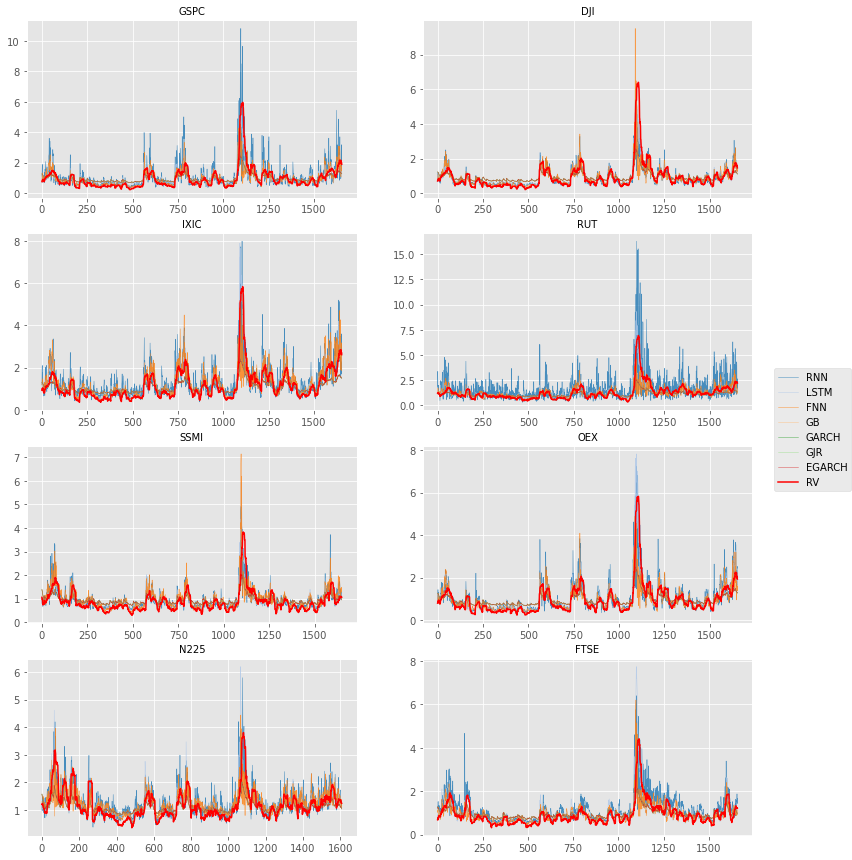
\includegraphics[width = 12.4cm]{figures/VOLA_FIGURS.png}
    \caption{Conditional Volatilities on the Test Set and Realized Volatility}
    \label{fig:my_label}
\end{figure}

\begin{figure}
    \centering
    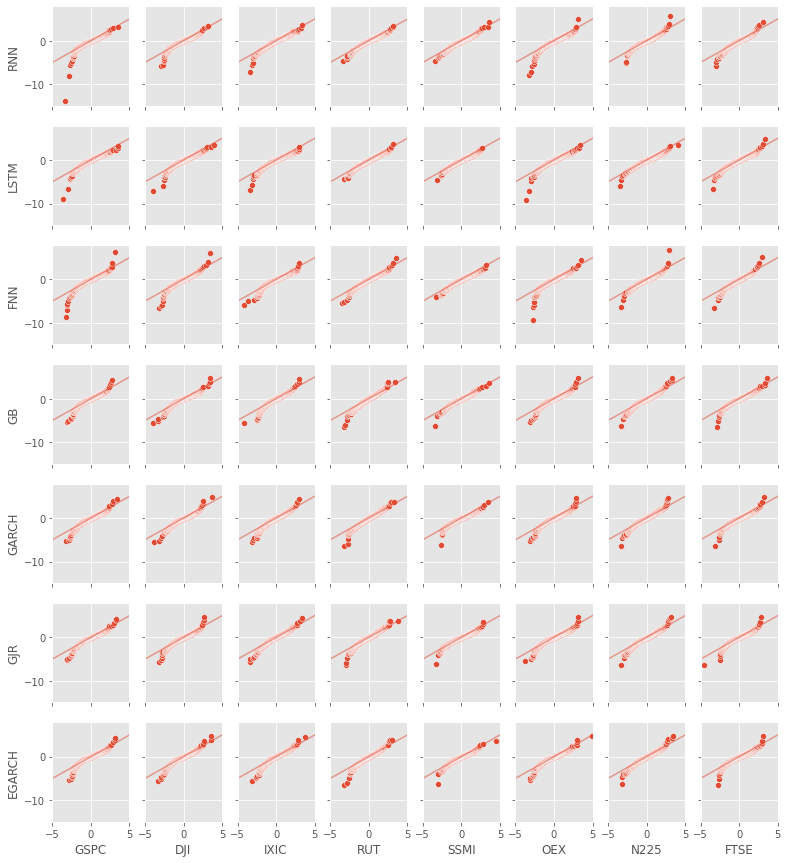
\includegraphics[width = 13.4cm]{figures/QQ_plot.png}
    \caption{ Q-Q Plots of the Residuals}
    \label{fig:my_label}
\end{figure}

%---------------------------------------------------------------

\printbibliography

\end{document}